\documentclass[11pt,a4paper]{article}
\usepackage[UTF8]{ctex}
\usepackage{amsmath,amssymb,amsthm,mathtools}
\usepackage{graphicx}
\usepackage{tikz}
\usetikzlibrary{shapes.geometric, arrows.meta, positioning, calc, backgrounds, fit, shadows}
\usepackage{geometry}
\geometry{left=2.5cm,right=2.5cm,top=2.8cm,bottom=2.8cm}
\usepackage{xurl}
\usepackage{hyperref}
\hypersetup{
    colorlinks=true,
    linkcolor=black,
    citecolor=blue!80!black,
    urlcolor=blue!80!black
}
\usepackage{booktabs}
\usepackage{array}
\usepackage[numbers,sort&compress]{natbib}
\usepackage{titlesec}
\usepackage{caption}
\captionsetup{labelsep=space,font={small,bf}}

% Custom section formatting according to Chinese journal style using titlesec
\titleformat{\section}{\raggedright\heiti\zihao{4}\bfseries}{\thesection}{1em}{}
\titleformat{\subsection}{\raggedright\heiti\zihao{5}\bfseries}{\thesubsection}{1em}{}
\titleformat{\subsubsection}{\raggedright\heiti\zihao{5}}{\thesubsubsection}{1em}{}
\titlespacing*{\section}{0pt}{1.5ex plus .2ex minus .2ex}{1ex plus .2ex}
\titlespacing*{\subsection}{0pt}{1.2ex plus .2ex minus .2ex}{0.8ex plus .2ex}
\titlespacing*{\subsubsection}{0pt}{1.0ex plus .2ex minus .2ex}{0.6ex plus .2ex}

% Theorem environments
\theoremstyle{plain}
\newtheorem{theorem}{定理}
\newtheorem*{theorem5R}{定理 5R（定理 5 的时变自回归扩展）}
\newtheorem{lemma}{引理}
\newtheorem{corollary}{推论}
\theoremstyle{definition}
\newtheorem{definition}{定义}

% Remove LaTeX default proof square box (keep only Chinese '证毕。')
\renewcommand{\qedsymbol}{}

% TikZ colors
\definecolor{navyMain}{RGB}{24, 48, 89}
\definecolor{tealMain}{RGB}{16, 124, 138}
\definecolor{coralMain}{RGB}{210, 85, 40}
\definecolor{slateGray}{RGB}{65, 80, 100}
\definecolor{cardTealBg}{RGB}{242, 251, 252}
\definecolor{cardBlueBg}{RGB}{243, 247, 254}
\definecolor{cardOrangeBg}{RGB}{255, 247, 242}
\definecolor{cardGrayBg}{RGB}{248, 250, 253}
\definecolor{panelBorderBlue}{RGB}{175, 200, 230}
\definecolor{panelBorderOrange}{RGB}{245, 190, 160}

\begin{document}

% Title (without author placeholders)
\begin{center}
    \vspace*{0.5em}
    {\zihao{2}\heiti\bfseries 传染病传播动力学的可预测视界、理论极限与实证研究} \\[1.8em]
\end{center}

% Abstract & Keywords Box
\noindent{\heiti\bfseries 摘要：}传染病前瞻预测在流行阈值附近常发生系统性精度衰退，构成了计算流行病学与公共卫生预警领域长期存在的理论瓶颈。本文基于负二项分支过程这一基本数据生成模型，推导出了前瞻预测相对均方误差的正交分解与可预测视界解析映射。研究将预测误差解耦为微观生灭内在相对方差与外在参数推断几何级放大项，导出了离散整年代际视界非零充要判据（要求单代前瞻误差满足 $\text{relMSE}^2(1) \le \tau^2$）与一阶连续渐近松弛闭式解 $h^*$，并揭示了当容忍度低于渐近方差饱和极限时的纯内在随机性视界硬上限 $h^*_{\text{stoch}}$。在此基础上，本文确立了四项核心理论性质：第一，在负二项似然下推导出参数推断的 Cram\'er--Rao 方差下界，确立了判别暴发超临界增长的刚性样本量下限（在备择假设 $R=1.1$ 处严格方差界需 231 例独立病例，80\% 功效单侧检验需 1,428 例；零假设边界 $R=1$ 处分别对应约 200 例与 1,237 例）；第二，刻画了有限种群带反射截断的扩散近似平稳态，揭示了近临界相变过渡窗口（标度为 $|\varepsilon| \lesssim O(N^{-1/2})$）内拟平稳长尾涨落导致预测视界发生临界退化；第三，推导出了宏观聚合发病数的 $h/k$ 尺度无关对数方差地板与平稳自回归增长率下的方差累积律；第四，机器学习基准实验在无偏分支似然设定下严格验证了 Cram\'er--Rao 信息论下界的不可逾越性。基于美国疾病预防控制中心（CDC）三大呼吸道传染病七大典型流行阶段的实测数据，在单流行季自然物理截断下，理论预测视界精确根为 4.7--16.0 周（纯数学外推根为 4.7--49.4 周）；完全预测误差预算核算显示，未归因闭合余项占 63.2\%--86.0\%；滚动样本外预测验证进一步证实了真实预测技能在 1--4 周后衰退至持续性基线水平，确立了理论上限与现实操作视界的双层层次结构。本研究表明临界失效是随机生灭动力学与信息论规律决定的内在客观约束，为公共卫生监测预警提供了坚实的数理基准。

\vspace{0.8em}
\noindent{\heiti\bfseries 关键词：}传染病预测；可预测视界；分支过程；群体内在随机性；近临界动力学；Fisher 信息量；模型误配

\vspace{1.5em}


\section*{0\quad 引言}
\addcontentsline{toc}{section}{0\quad 引言}

传染病前瞻性预测在不同流行阶段的表现存在显著差异。在已进入稳定暴发的波次中，动力学模型通常能在数周前置时间内保持较高准确度；然而一旦疫情接近流行阈值（即基本再生数 $R \approx 1$ 的临界点），预测性能便发生断崖式退化\citep{scarpino2019predictability, reich2019collaborative}。针对季节性流感、登革热和 COVID-19 的协同预测评估项目\citep{mcgowan2019collaborative, johansson2019open, cramer2022evaluation}反复证实了这一普遍现象。尽管基于加权区间评分的标准化评估方法\citep{bracher2021evaluating}能够量化预测误差，但仍无法从动力学机理上解释预测精度上限的决定规律以及失效边界的数学成因。类似地，早期增长率的实时贝叶斯与似然估计在流行阈值附近精度显著下降\citep{bettencourt2008real, fraser2007estimating}；动力学模型与概率预测算法亦表现出类似气象动力系统前瞻预测的视界衰减效应\citep{moran2016epidemic, castro2020predictability, funk2018realtime, held2017probabilistic}。例如在 RAPIDD 埃博拉多模型预测评估项目中，暴发初期与转折点各参与模型的预测分散度极大且难以稳健超越基线外推\citep{viboud2018rapidd}。实时预测前瞻评述亦指出，近临界与数据稀疏状态是各建模路线面临的普遍失效诱因\citep{desai2019realtime}。

阈值附近的参数估计存在固有偏差且方差急剧发散\citep{britton2019estimation}，显著放大了分支过程与随机动力学生灭过程固有的群体内在随机性\citep{bartlett1957measles, athreya1972branching}。在生物数学与疾病生态学领域，有限随机宿主群体中是否存在明确的病原体输入暴发阈值（Invasion Threshold），长期以来是重要的基础理论问题\citep{lloydsmith2005should}。在生物预测领域，Petchey 等\citep{petchey2015ecological}系统阐述了利用精度容忍度定义可预测视界的分析框架；Drake\citep{drake2006limits}基于随机生灭过程论证了接触随机性设定了暴发规模精度的根本极限；Penn 等\citep{penn2023intrinsic}进一步指出分支过程中偶然不确定性与认知不确定性共同主导前瞻风险；Johnson 等\citep{johnson2021disease}则分析了超扩散过离散对再生数推断精度的约束。随机流行病过程的临界行为（类似于统计物理中的动力学渗流\citep{grassberger1983critical}）深刻约束着预测系统的信息提取边界。经验证据表明近临界动力学与超临界动力学存在本质差异，但现有研究多侧重于静态再生数反演或特定算法的经验对比，尚未在统一的负二项分支过程第一性原理框架下，将再生数 $R$、超扩散离散度 $k$、初始暴发规模 $I_0$ 与参数不确定性 $\delta R$ 显式耦合，以定量解析求解可预测视界的时间跨度。

可预测视界（Predictability Horizon）的概念为刻画疫情演化的时间尺度提供了自然基准。代间隔定义为传播链中连续两代感染之间的时间间隔，构成了流行病学生灭过程的时间度量基准。分支过程每经历一个代间隔即向前推进一步，因此以代数计的预测跨度 $h$ 对应的时间约为 $h \mu_g$，其中 $\mu_g$ 为平均代间隔\citep{wallinga2007generation}。在实际监测中，$\mu_g$ 及代间隔分布的经验估计往往伴随不可忽视的不确定性。代间隔分布的设定偏差会同时影响再生数估计与前向投影精度\citep{park2020forward}。针对新发病原体的代间隔估计仍在持续完善\citep{nishiura2009generation, hakki2022serial}，本文在实证章节检验了视界计算对此类参数变动的敏感性。视界 $h^*$ 首先以代数表达，旨在不同代间隔特性的传染病之间建立标准化的比较尺度。

这一理论难题在公共卫生实践中带来了现实挑战。当实时预测出现偏差（例如预测指数增长却出现平台期，或过早判定疫情消退却遭遇反弹）时，其成因可能源于模型设定偏误、监测数据不足，或是系统内在的动力学随机性。若缺乏严格的数理分解，决策部门将难以厘清：究竟应投入算力改进算法、增加监测采样，还是承认系统在该阶段已超出理论可预测范围？若在信息论不可预测盲区盲目发布点预测，失准将严重削弱预警决策的科学性。为此，本文提供了严格的解析推导方法：针对不同暴发阶段，推导由 $R$、$k$、$I_0$ 与 $\delta R$ 决定的最小理论均方误差，并给出可预测视界 $h^*$ 的闭式解。在超出该理论界限后，任何算法优化均无法在给定机理假设下进一步提升预测能力。

控制子代方差离散程度的参数 $k$ 是生物数学与应用统计建模的核心对象。对呼吸道传染病而言，传播过程通常呈现显著的超扩散（Superspreading）过离散特征：极少数超级传播者贡献了绝大部分续发病例\citep{lloyd-smith2005superspreading, endo2020overdispersion}。由于负二项分布的单代子代方差 $\sigma^2 = R + R^2/k$ 随 $k$ 减小而无界增大，过离散直接抬高了预测的不可约方差地板。此外，在流行阈值附近估计 $k$ 面临严重的信噪比不足问题，这一耦合机制在本文的实证与敏感性分析中得到了定量检验。

需要明确指出，本文涉及的分支过程二阶矩\citep{athreya1972branching, bartlett1957measles}、弱超临界建群概率\citep{o2013theory}、有限种群 SIS 拟平稳标度\citep{nasell1999quasi, dolgoarshinnykh2006critical}、负二项 Fisher 信息\citep{johnson2021disease, lloyd2007maximum}以及时间序列累积方差律均属经典随机过程与数理统计的基础构件。本文的核心增量贡献在于：据作者所知，首次在统一的负二项分支过程第一性原理框架下，将五维动力学参数 $(R, k, I_0, \delta R, \tau)$ 显式映射为可预测领先时间的解析解 $h^*$ 与数值精确根 $h^*_{\text{exact}}$；严格给出了离散非零视界的充要判据与纯随机性视界上限 $h^*_{\text{stoch}}$；并通过完全误差预算核算与滚动样本外预测验证，揭示了由内在机制理论上限与实测外生闭合余项共同决定的双层层次结构。

这一理论推导的实用价值体现在三个明确方面：第一是多源噪声的非线性耦合：群体内在随机性、参数估计不确定性与近临界拟平稳涨落在 $h^*$ 中呈现乘积与开方耦合，单一来源分析无法刻画此种联合效应；第二是定量标定能力：闭式公式为具体参数组合 $(R,k,I_0,\delta R)$ 提供了明确的数值视界 $h^*$，克服了以往文献仅有定性描述的局限；第三是事前评估基准：$h^*$ 将预测有效性转化为事前可计算的定量指标，能够与区间格式评分标准\citep{bracher2021evaluating}无缝衔接。

本文的结构安排如下：第 1 节系统回顾相关文献背景与研究进展；第 2 节建立基于负二项分支过程的理论模型，给出引理 1、引理 2 的严格数学证明，推导均方误差正交分解、闭式视界上限及核心推论；第 3 节介绍高通量蒙特卡洛模拟设计与机器学习算法基准检验；第 4 节呈现美国 CDC 三大呼吸道传染病七大典型阶段的真实视界测算与五项完全误差分解实证结果；第 5 节深入探讨公共卫生决策启示与局限性；第 6 节总结全文主要结论。

\section{研究回顾}

\subsection{协同预测项目与系统性评估}
多模型协同预测评估项目已在大规模真实疫情中完整记录了临界失效模式。FluSight 流感预测\citep{mcgowan2019collaborative}、RAPIDD 埃博拉多模型评估\citep{viboud2018rapidd}、登革热预测计划\citep{johansson2019open}与 COVID-19 协同预测中心\citep{cramer2022evaluation}系统性比较了数十个团队的模型表现，一致发现在近临界阶段模型预测技能普遍降至甚至低于简单的基线外推模型，但始终缺少统一的动力学方程将流行病学参数与可达精度极限直接相连。近期，White 与 Le{\'o}n\citep{white2026forecastability}将时间序列可预测性指标与 Forecast Hub 实际多周预报技能进行了经验对照。然而，评估方法论（如加权区间评分 WIS\citep{bracher2021evaluating}）通常侧重于事后评测，缺少直接源自底层生灭动力学的第一性原理理论视界 $h^*$ 作为前置分析基准。本文推导的视界公式为量化经验预测技能衰减提供了理论物理参照。

\subsection{分支过程与更新方程}
分支过程与更新方程作为传染病动力学推断的基石具有深厚理论渊源。负二项子代分布的 Galton--Watson 过程\citep{harris1963branching, athreya1972branching, jagers1975branching}与连续时间更新方程\citep{wallinga2004different, wallinga2007generation, cori2013framework}为实时 $R_t$ 估计\citep{abbott2020epinow2, gostic2020practical}与早期增长率推断\citep{bettencourt2008real}提供了标准的统计似然基础。近年来，研究者广泛将离散度参数 $k$ 作为超扩散程度的度量指标\citep{lloyd-smith2005superspreading, endo2020overdispersion}，但尚未有研究推导出连接 $(R, k, I_0, \delta R)$ 到定量预测视界 $h^*$ 的闭式解。经典的个体与家庭再生数估计\citep{fraser2007estimating}侧重于静态点估计，本文则将分支过程结构推展至动态预测的误差下界分析。

\subsection{临界现象与拟平稳动力学}
统计物理中的临界相变与灭绝动力学为描述近临界流行病过程提供了精细的随机分析工具。分支过程的拟平稳分布（Quasi-Stationary Distribution, QSD）\citep{darroch1965quasi}、临界慢化现象\citep{kessler2007extinction}、Logistic 扩散逼近\citep{ethier1986markov}与动力学渗透理论\citep{grassberger1983critical}刻画了有限种群中当 $|\varepsilon|=|R-1| \ll 1$ 时的长尾涨落与建群概率（Establishment Probability）。Britton 与 Tomba\citep{britton2019estimation}分析了阈值附近的参数估计偏差。有限种群阈值的生物数学争论\citep{lloydsmith2005should}指出随机干扰抹平了确定性 $R_0 = 1$ 的分界线；N{\aa}sell\citep{nasell1999quasi}与 Dolgoarshinnykh 和 Lalley\citep{dolgoarshinnykh2006critical}严格推导了随机流行病模型在临界态附近的扩散标度与拟平稳渐近。本文定理 3 显式给出了该临界窗口宽度 $|\varepsilon| \lesssim O(N^{-1/2})$，并揭示了拟平稳大变异系数引发的预测视界压缩机制。

\subsection{传染病预测中的机器学习理论边界}
近年来，机器学习与深度学习被广泛应用于传染病预测任务，从流感预测基准\citep{reich2019collaborative, ray2023comparing}到多源正则化机器学习\citep{colubri2019machine}与深度自回归网络\citep{salinas2020deepar}。然而现有文献大多聚焦于经验性能对比（即“哪个模型在特定数据集上表现更优”），极少追问其相对于理论最小均方误差下界的位置。LightGBM 等梯度提升树\citep{ke2017lightgbm}与多层感知机（MLP）虽展现出强大的非线性拟合能力，但在无偏数据生成机制下能否突破理论辨识极限此前缺乏严格测试。

值得注意的是，现有关于流行病学信息论极限的研究主要集中于参数推断与实时追踪，例如 Parag 与 Donnelly\citep{parag2022fundamental} 利用滤波与平滑后验下的 Fisher 信息与 Cram\'er--Rao 下界，系统探讨了实时推断复发风险时的内在延迟与信息提取极限；而确定性动力系统视角下的预测视界研究（如 Castro 等\citep{castro2020predictability}）则侧重于流行病峰值转折点的不可预测性约束。据作者所知，现有研究尚未建立连接五维动力学参数 $(R, k, I_0, \delta R, \tau)$ 到定量时间视界的闭式解。本文在统一的负二项分支框架中导出了可预测视界的显式表达，为判断算法改进是逼近了物理数理天花板还是仅在优化局部拟合提供了客观基准。

\section{理论与方法}

\subsection{数据来源与预处理}\label{sec:data}
为实证检验理论推导在真实暴发情境中的适用性，本文采用了美国疾病预防控制中心（CDC）公开发布的国家级周度聚合监测序列（数据访问快照为 2026 年 3 月公开版）。监测目标序列定义如下：COVID-19 采用 COVID Data Tracker 国家级每周确诊发病数（Confirmed Weekly Cases）；季节性流感采用 FluView 临床实验室确诊阳性标本周数（Clinical Lab Confirmed Positive Influenza Specimens）；RSV 采用 NREVSS 实验室 PCR 检测阳性周数（PCR-Confirmed RSV Detections）。实证分析严格覆盖七大典型流行阶段：COVID-19 Delta 暴发期（2021-W26 至 2021-W30）、Omicron 达峰期（2021-W49 至 2022-W03）、JN.1 流行期（2023-W48 至 2024-W02）；季节性流感 2022--23 流行季（2022-W40 至 2022-W44）、2024--25 流行季（2024-W40 至 2024-W44）；RSV 2024--25 流行季（2024-W40 至 2024-W44）及 2025--26 流行季（2025-W40 至 2025-W44）。历史回测基于回填固化后的最终序列（Finalized Data Vintage），作为评估理论可预测性物理上限的基准。数据预处理以各阶段起步期连续 4 周数据作为推断窗口，采用滑动窗口对数线性回归估计净增长率与再生数 $R$ 及其标准误 $\delta R$，结合负二项二阶矩法求解宏观过度离散度 $k_{\text{agg}}$，初始发病规模 $I_0$ 取窗口平均周发病数；目标容忍度设为 $\tau = 0.5$（对应相对均方根误差 50\%），采用 2,000 次参数化 Bootstrap 重抽样（固定随机种子 42）评估置信区间。

\subsection{模型设定与基础引理证明}

本文在微观层面采用标准 Galton--Watson 负二项分支过程作为基础数据生成模型，图~\ref{fig:framework_cn}系统展示了从双源随机性输入到相对均方误差正交分解，再到预测视界闭式解与核心推论的理论推导脉络。

\begin{figure}[htbp]
\centering
\resizebox{0.96\textwidth}{!}{%
\begin{tikzpicture}[
    >=Stealth,
    font=\sffamily,
    card/.style={
        rectangle, rounded corners=6pt, draw=#1, fill=white, line width=1.1pt,
        inner sep=8pt, align=center, drop shadow={opacity=0.07, shadow xshift=1pt, shadow yshift=-1.5pt}
    },
    subcard/.style={
        rectangle, rounded corners=4pt, draw=#1, line width=0.8pt,
        inner sep=5pt, align=center
    },
    panel/.style={
        rectangle, rounded corners=8pt, draw=#1, line width=0.9pt, dashed, inner sep=10pt, fill opacity=0.35
    },
    arrow/.style={
        ->, line width=1.3pt
    }
]

% 1. TIER 1: INPUT NOISE SOURCES
\node[card=tealMain, fill=cardTealBg, text width=6.3cm] (demo) {
    \textbf{\large\color{tealMain} 群体内在随机性（微观统计涨落）}\\[4pt]
    \footnotesize 生成机制：负二项分支过程 (子代 $\sim \text{NB}(R, k)$)\\[4pt]
    \textbf{\small 不可约误差地板（引理 2 / 定理 1）：}\\[3pt]
    $\text{CV}^2(h) = \dfrac{(1+R/k)(1-R^{-h})}{I_0(R-1)} \xrightarrow{h\to\infty} \dfrac{1+R/k}{I_0(R-1)}$
};

\node[card=navyMain, fill=cardBlueBg, text width=6.3cm, right=1.2cm of demo] (param) {
    \textbf{\large\color{navyMain} 参数不确定性（外在推断误差）}\\[4pt]
    \footnotesize 观测推断：监测窗口估计量 $\hat{R} \sim \mathcal{N}(R, \delta R^2)$\\[4pt]
    \textbf{\small 几何级放大项（引理 3）：}\\[3pt]
    $P(h) = \dfrac{\mathbb{E}[(\hat{R}^h - R^h)^2]}{R^{2h}} \approx \left(\dfrac{h\,\delta R}{R}\right)^2$
};

% 2. TIER 2: ORTHOGONAL ERROR DECOMPOSITION
\node[card=slateGray, fill=cardGrayBg, text width=12.8cm, below=1.5cm of $(demo.south)!0.5!(param.south)$] (decomp) {
    \textbf{\large\color{navyMain} 相对均方误差严格正交分解（定理 1 与单调性定理 2）}\\[6pt]
    \Large $\text{relMSE}^2(h) = \underbrace{\text{CV}^2(h)}_{\text{\normalsize 内在随机性地板}} + \underbrace{P(h)}_{\text{\normalsize 参数不确定性放大}} \le \tau^2$\\[5pt]
    \small\color{slateGray} （在分支过程与无偏估计独立性假定下正交无交叉项，且随前置时间 $h$ 严格单调递增）
};

% 3. TIER 3: HORIZON CEILING & LIMIT THEOREMS
\node[card=coralMain, fill=cardOrangeBg, text width=13.8cm, below=2.6cm of decomp.south] (horizon) {
    \textbf{\Large\color{coralMain} 理论可预测视界上限与数理界限（$h^*$）}\\[7pt]
    
    \begin{tikzpicture}[node distance=0.25cm]
        \node[subcard=coralMain, fill=white, text width=6.3cm, inner sep=4.5pt] (hmain) {
            \textbf{\small\color{coralMain} 主视界闭式公式（$R > 1$ 超临界）}\\[3pt]
            \scalebox{0.85}{$\boxed{\rule[-7pt]{0pt}{20pt}\, h^*_{\text{周}} \approx \dfrac{\mu_g}{7} \cdot \dfrac{R}{\delta R}\sqrt{\tau^2 - \dfrac{1+R/k}{I_0(R-1)}} \,}$}\\[3pt]
            \scriptsize （$\tau$ 为目标相对误差容忍度）
        };
        \node[subcard=coralMain, fill=white, text width=6.3cm, inner sep=4.5pt, right=0.25cm of hmain] (hcrit) {
            \textbf{\small\color{coralMain} 近临界正根解析解（推论 1：$R \to 1$）}\\[3pt]
            \scalebox{0.85}{$\boxed{\rule[-7pt]{0pt}{20pt}\, h^*_{\text{gen}} = \dfrac{\sqrt{b^2+4\delta R^2\tau^2}-b}{2\delta R^2} \,}$}\\[3pt]
            \scriptsize （其中 $b = \dfrac{1+1/k}{I_0}$ 为初始群体离散项）
        };
    \end{tikzpicture}\\[8pt]
    
    \begin{tikzpicture}[node distance=0.25cm]
        \node[subcard=coralMain, fill=white, text width=3.8cm, inner sep=4.5pt] (t3) {
            \textbf{\color{coralMain} 近临界相变特征 (定理 3)}\\[2pt]
            \scriptsize 拟平稳扩散涨落主导\\
            $|\varepsilon| \lesssim O(N^{-1/2}) \implies h^* \to 0$\\
            推论 2 建群率 $s \approx \frac{2\varepsilon}{R(1+R/k)}$
        };
        \node[subcard=coralMain, fill=white, text width=3.8cm, inner sep=4.5pt, right=0.25cm of t3] (t4) {
            \textbf{\color{coralMain} 信息论辨识下限 (定理 4)}\\[2pt]
            \scriptsize Cramér--Rao 最小病例数\\
            $C \ge \frac{R^2(1/R+1/k)}{\varepsilon^2} \approx 231$\\
            80\% 功效需 $C \ge 1,428$
        };
        \node[subcard=coralMain, fill=white, text width=3.8cm, inner sep=4.5pt, right=0.25cm of t4] (t5) {
            \textbf{\color{coralMain} 五项完全实测预算 (定理 5/5R)}\\[2pt]
            \scriptsize 五项完全正交分解\\
            $\text{relMSE}^2 = \text{CV}^2 + \mathcal{E}_{\text{drift}} + P$\\
            $+ \mathcal{E}_{\text{cross}} + \mathcal{E}_{\text{misspec}}$
        };
    \end{tikzpicture}
};

% 4. CONNECTING FLOW ARROWS
\draw[arrow, draw=tealMain] (demo.south) -- (demo.south |- decomp.north)
    node[midway, left=2pt, font=\bfseries\small\color{tealMain}] {内在机制贡献};

\draw[arrow, draw=navyMain] (param.south) -- (param.south |- decomp.north)
    node[midway, right=2pt, font=\bfseries\small\color{navyMain}] {外在推断贡献};

\node[fill=white, inner sep=3.5pt, rounded corners=3pt, draw=coralMain, line width=0.8pt, font=\bfseries\small\color{coralMain}, below=0.35cm of decomp.south] (critBadge) {首次达到目标误差容忍度 $\text{relMSE}(h^*) = \tau$};

\draw[arrow, line width=1.8pt, draw=coralMain] (decomp.south) -- (critBadge.north);
\draw[arrow, line width=1.8pt, draw=coralMain] (critBadge.south) -- (horizon.north);

% 5. BACKGROUND CONTAINERS
\begin{scope}[on background layer]
    \node[panel=panelBorderBlue, fill=cardBlueBg, fit=(demo) (param), 
          label={[anchor=south west, font=\bfseries\small\color{navyMain}, xshift=4pt, yshift=2pt]north west:【阶段 I：双源随机性底层生成机制】}] {};
          
    \node[panel=panelBorderOrange, fill=cardOrangeBg, fit=(horizon), 
          label={[anchor=south west, font=\bfseries\small\color{coralMain}, xshift=4pt, yshift=2pt]north west:【阶段 II：理论界限定量输出与公卫决策基准】}] {};
\end{scope}

\end{tikzpicture}%
}
\caption{\textbf{传染病传播动力学与预测视界理论推导原理图。}展示双源随机性输入（群体内在随机性地板与外在参数推断放大）、预测均方误差正交分解（定理 1 与单调性定理 2）以及由此导出的理论可预测视界上限 $h^*$（含超临界闭式与近临界推论 1 解析解）和核心理论推论（定理 3 临界慢化坍塌、定理 4 信息论辨识下限与定理 5/5R 时变误差预算）。}
\label{fig:framework_cn}
\end{figure}

模型设立以下标准动力学与统计推断假定：
\begin{itemize}
\item[(A1)] 子代分布：各感染个体产生的二代病例数独立同分布服从负二项分布 $\text{NB}(R, k)$，均值为基本再生数 $R$，离散度为 $k$，单代子代方差 $\sigma^2 = R + R^2/k$。
\item[(A2)] 传播稳定性：在预测视界 $h$ 内 $R$ 保持恒定（时变与漂移推广见定理 5 与定理 5R）。
\item[(A3)] 时间尺度：平均代间隔为 $\mu_g$，代际预测步长 $h$ 对应的时间跨度为 $T = \mu_g h$。
\item[(A4)] 统计独立性：监测窗口参数估计量 $\hat{R}$ 条件独立于预测期内的微观随机传播实现。
\end{itemize}

以下给出分支过程均值与方差的一阶及二阶矩递推引理及其严格证明。

\begin{lemma}[分支过程两阶段矩递推]\label{lem:branch_moments}
设初始发病人数为 $Z_0 = I_0$，在假定 (A1) 下，第 $h$ 代新发感染人数（发病规模）$Z_h$ 的期望与方差分别为：
\begin{equation}
\mathbb{E}[Z_h] = I_0 R^h,
\end{equation}
\begin{equation}
\text{Var}(Z_h) = I_0 \sigma^2 R^{h-1} \frac{R^h - 1}{R - 1}, \quad (R \neq 1).
\label{eq:lem1_var}
\end{equation}
\end{lemma}

\begin{proof}
根据分支过程定义，第 $n$ 代发病人数可表示为上一代个体的后代总和：
\begin{equation}
Z_n = \sum_{j=1}^{Z_{n-1}} X_{n-1, j},
\end{equation}
其中 $\{X_{n-1, j}\}$ 独立同分布于负二项分布，满足 $\mathbb{E}[X] = R$，$\text{Var}(X) = \sigma^2 = R + R^2/k$。

由全期望公式（Law of Total Expectation）：
\begin{equation}
\mathbb{E}[Z_n \mid Z_{n-1}] = Z_{n-1} \mathbb{E}[X] = R Z_{n-1}.
\end{equation}
两边取无条件期望得 $\mathbb{E}[Z_n] = R \mathbb{E}[Z_{n-1}]$。由初始条件 $\mathbb{E}[Z_0] = I_0$，递推直接解得 $\mathbb{E}[Z_h] = I_0 R^h$。

对于方差，应用全方差公式（Law of Total Variance / Eve's Law）：
\begin{align}
\text{Var}(Z_n) &= \mathbb{E}[\text{Var}(Z_n \mid Z_{n-1})] + \text{Var}(\mathbb{E}[Z_n \mid Z_{n-1}]) \notag \\
&= \mathbb{E}[Z_{n-1} \sigma^2] + \text{Var}(R Z_{n-1}) \notag \\
&= \sigma^2 \mathbb{E}[Z_{n-1}] + R^2 \text{Var}(Z_{n-1}) \notag \\
&= \sigma^2 I_0 R^{n-1} + R^2 \text{Var}(Z_{n-1}).
\end{align}
记 $V_n = \text{Var}(Z_n)$，将上述一阶非齐次线性递推关系两端同除以 $R^{2n}$：
\begin{equation}
\frac{V_n}{R^{2n}} - \frac{V_{n-1}}{R^{2(n-1)}} = \frac{\sigma^2 I_0}{R^{n+1}}.
\end{equation}
对 $n = 1, 2, \dots, h$ 累加求和（利用初始条件 $V_0 = \text{Var}(I_0) = 0$）：
\begin{equation}
\frac{V_h}{R^{2h}} = \sigma^2 I_0 \sum_{n=1}^h R^{-(n+1)} = \frac{\sigma^2 I_0}{R^2} \cdot \frac{R^{-1}(1 - R^{-h})}{1 - R^{-1}} = \frac{\sigma^2 I_0 (R^h - 1)}{R^{h+1}(R - 1)}.
\end{equation}
两端同乘以 $R^{2h}$，即严格导出：
\begin{equation}
\text{Var}(Z_h) = I_0 \sigma^2 R^{h-1} \frac{R^h - 1}{R - 1}.
\end{equation}
证毕。
\end{proof}

\begin{lemma}[群体内在变异系数与方差地板]\label{lem:cv_floor}
第 $h$ 代发病人数的相对方差（变异系数平方 $\text{CV}^2(h)$）具有严格闭式解：
\begin{equation}
\text{CV}^2(h) = \frac{\text{Var}(Z_h)}{(\mathbb{E}[Z_h])^2} = \frac{(1 + R/k)(1 - R^{-h})}{I_0(R - 1)},
\label{eq:cv_floor}
\end{equation}
该式从 $h=0$ 处的 $\text{CV}^2(0)=0$ 出发，关于前置步长 $h$ 严格单调递增。在单代首步（$h=1$）处，其严格取值为 $\text{CV}^2(1) = \frac{1+R/k}{I_0 R}$；当 $h \to \infty$ 时收敛至渐近方差饱和极限 $\text{CV}^2_\infty \equiv \frac{1 + R/k}{I_0(R - 1)}$。当 $R \to 1$ 时，其极限连续延拓为线性累积形式 $h(1+1/k)/I_0$。
\end{lemma}

\begin{proof}
将引理 1 中的方差表达式代入相对方差定义，并利用 $\sigma^2 = R(1 + R/k)$：
\begin{align}
\text{CV}^2(h) &= \frac{I_0 R(1 + R/k) R^{h-1} \frac{R^h - 1}{R - 1}}{(I_0 R^h)^2} \notag \\
&= \frac{I_0 (1 + R/k) R^h (R^h - 1)}{I_0^2 R^{2h} (R - 1)} \notag \\
&= \frac{(1 + R/k)(1 - R^{-h})}{I_0(R - 1)}.
\end{align}
对于 $R > 1$，由于 $R^{-h}$ 随 $h$ 单调递减趋于 0，因此 $1 - R^{-h}$ 严格单调递增趋于 1，直接证明了单调性与渐近极限。

对于近临界极限 $R \to 1$，由于分母 $R - 1 \to 0$ 且分子 $1 - R^{-h} \to 0$，应用洛必达法则（L'H\^opital's Rule）对 $R$ 求导：
\begin{equation}
\lim_{R \to 1} \frac{1 - R^{-h}}{R - 1} = \lim_{R \to 1} \frac{-(-h) R^{-h-1}}{1} = h.
\end{equation}
代入即得 $\lim_{R \to 1} \text{CV}^2(h) = \frac{h(1 + 1/k)}{I_0}$。该极限亦可直接通过在 $R=1$ 下对负二项单代方差 $1+1/k$ 进行 $h$ 代线性累加求和导出，证明了极限处的一阶连续性。
证毕。
\end{proof}

\begin{lemma}[参数不确定性的几何级放大项]\label{lem:param_amplification}
在流行病学参数推断中，再生数估计量严格满足非负支撑 $\hat{R} \in (0, \infty)$（在对数连接广义线性回归或更新方程下，对数再生数满足渐近正态性 $\log \hat{R} \sim \mathcal{N}(\log R, (\delta R / R)^2)$，对应对数正态估计分布；或在截断正态模型 $\hat{R} \sim \mathcal{N}(R, \delta R^2)\mathbf{1}_{\hat{R}>0}$ 下，当信噪比 $R/\delta R \ge 15.9$ 时，负尾截断概率 $\Phi(-15.9) < 10^{-56}$，在实数域严格良定）。在假定其条件独立于预测期微观过程的前提下，参数估计误差导致的相对均方误差贡献项为：
\begin{equation}
P(h; R, \delta R) = \frac{\mathbb{E}[(I_0 \hat{R}^h - \mathbb{E}[Z_h])^2]}{(\mathbb{E}[Z_h])^2} = \frac{\mathbb{E}[(\hat{R}^h - R^h)^2]}{R^{2h}} = \text{Var}\left[\left(\frac{\hat{R}}{R}\right)^h\right] + \left\{\mathbb{E}\left[\left(\frac{\hat{R}}{R}\right)^h\right] - 1\right\}^2.
\end{equation}
当相对累积参数误差较小时（$h \delta R / R \ll 1$），经一阶 Delta 线性化展开（忽略 Jensen 偏置平方阶项）可得领先阶解析近似：
\begin{equation}
P(h; R, \delta R) \approx \left(\frac{h\,\delta R}{R}\right)^2.
\end{equation}
\end{lemma}

\begin{proof}
定义实函数 $f(r) = r^h$。在点 $r = R$ 处进行一阶泰勒展开可得 $f(\hat{R}) \approx f(R) + f'(R)(\hat{R}-R) = R^h + h R^{h-1}(\hat{R}-R)$。由此，前向误差的二阶期望展开为：
\begin{equation}
\mathbb{E}[(\hat{R}^h - R^h)^2] \approx \mathbb{E}[(h R^{h-1}(\hat{R}-R))^2] = h^2 R^{2h-2} \text{Var}(\hat{R}) = h^2 R^{2h-2} \delta R^2.
\end{equation}
两端同除以归一化因子 $R^{2h}$，直接证得 $P(h; R, \delta R) \approx (h\,\delta R/R)^2$。
证毕。
\end{proof}

\subsection{相对均方误差分解与预测视界定理}

\begin{theorem}[预测相对均方误差正交分解与可预测视界映射]\label{thm:horizon}
在假定 (A1)--(A4) 下，前瞻点预测 $\hat{Z}_h = I_0 \hat{R}^h$ 的相对均方误差满足严格正交分解：
\begin{equation}
\text{relMSE}^2(h) = \frac{\mathbb{E}[(\hat{Z}_h - Z_h)^2]}{(\mathbb{E}[Z_h])^2} = \text{CV}^2(h) + P(h; R, \delta R) = \frac{(1+R/k)(1-R^{-h})}{I_0(R-1)} + P(h; R, \delta R).
\label{eq:relmse_decomp}
\end{equation}
定义在目标相对误差容忍度 $\tau$ 下的离散代际可预测视界为 $h^*_{\text{gen}} = \max \{ h \in \mathbb{N} : \text{relMSE}^2(h) \le \tau^2 \}$。该预测视界满足以下核心判定与解析性质：
\begin{enumerate}
\item \textbf{非零视界充要判据}：系统存在有效正整数视界（$h^*_{\text{gen}} \ge 1$）当且仅当首步（$h=1$）前瞻相对均方误差满足：
\begin{equation}
\text{relMSE}^2(1) = \frac{1+R/k}{I_0 R} + \left(\frac{\delta R}{R}\right)^2 \le \tau^2.
\label{eq:h_exist_cond}
\end{equation}
若该式不成立，则表明首代微观涨落或参数初始不确定性已击穿容忍度，系统不存在正视界（$h^*_{\text{gen}} = 0$）。
\item \textbf{领先阶渐近连续松弛基准}：在超临界体制（$R > 1$）且预设容忍度高于渐近方差饱和极限（$\tau^2 > \text{CV}^2_\infty = \frac{1+R/k}{I_0(R-1)}$）时，采用极限方差近似 $1-R^{-h} \approx 1$ 与一阶 Delta 线性化，导出领先阶渐近闭式视界：
\begin{equation}
h^*_{\text{周}} \approx \frac{\mu_g}{7} \cdot \frac{R}{\delta R} \sqrt{\tau^2 - \frac{1+R/k}{I_0(R-1)}} \quad (\text{周}).
\label{eq:horizon_cn}
\end{equation}
\item \textbf{纯内在随机性视界上限}：当预设容忍度低于渐近饱和极限（$\tau^2 \le \text{CV}^2_\infty$，但满足式 (\ref{eq:h_exist_cond})）时，即便参数推断完全精确（$\delta R = 0$），纯内在生灭涨落亦将在有限步内触碰容忍边界，其严格纯随机视界上限为：
\begin{equation}
h^*_{\text{stoch}} = \frac{-\ln\left(1 - \frac{\tau^2 I_0(R-1)}{1+R/k}\right)}{\ln R}.
\label{eq:h_stoch_bound}
\end{equation}
在 $\delta R > 0$ 时，精确连续根 $h^*$ 严格满足 $1 \le h^* < h^*_{\text{stoch}}$，并由全有限步非线性隐式方程 $\text{CV}^2(h) + P(h) = \tau^2$ 唯一确定。
\end{enumerate}
\end{theorem}

\begin{proof}
对预测误差分子展开：
\begin{equation}
\hat{Z}_h - Z_h = (I_0 \hat{R}^h - \mathbb{E}[Z_h]) - (Z_h - \mathbb{E}[Z_h]).
\end{equation}
平方并取期望：
\begin{align}
\mathbb{E}[(\hat{Z}_h - Z_h)^2] &= \mathbb{E}[(I_0 \hat{R}^h - \mathbb{E}[Z_h])^2] + \mathbb{E}[(Z_h - \mathbb{E}[Z_h])^2] \notag \\
&\quad - 2\,\mathbb{E}[(I_0 \hat{R}^h - \mathbb{E}[Z_h])(Z_h - \mathbb{E}[Z_h])].
\end{align}
根据假定 (A4)，参数估计量 $\hat{R}$ 独立于预测期微观随机过程。虽然对于 $h > 1$，由 Jensen 不等式可知 $\mathbb{E}[\hat{R}^h] \ge (\mathbb{E}[\hat{R}])^h = R^h$（即非线性外推存在高阶正偏差，导致 $\mathbb{E}[I_0 \hat{R}^h - \mathbb{E}[Z_h]] \ne 0$），但由于居中微观扰动项严格满足 $\mathbb{E}[Z_h - \mathbb{E}[Z_h]] \equiv 0$，由独立变量积的期望性质可知交叉项严格为零：
\begin{equation}
\mathbb{E}[(I_0 \hat{R}^h - \mathbb{E}[Z_h])(Z_h - \mathbb{E}[Z_h])] = \mathbb{E}[I_0 \hat{R}^h - \mathbb{E}[Z_h]] \cdot \mathbb{E}[Z_h - \mathbb{E}[Z_h]] = \mathbb{E}[I_0 \hat{R}^h - \mathbb{E}[Z_h]] \cdot 0 = 0.
\end{equation}
两端同除以 $(\mathbb{E}[Z_h])^2 = (I_0 R^h)^2$，并代入引理 2 与引理 3 的结论，即严格证得正交分解式 (\ref{eq:relmse_decomp})。

关于判定性质：由于 $\text{CV}^2(h)$ 与 $P(h)$ 关于步长 $h$ 严格单调递增（定理 2），$\text{relMSE}^2(h)$ 为严格递增函数。因此 $h^*_{\text{gen}} \ge 1$ 当且仅当 $h=1$ 处未超标，代入引理 2 的 $h=1$ 取值即直接导出充要条件 (\ref{eq:h_exist_cond})。在 $\tau^2 > \text{CV}^2_\infty$ 时，将渐近饱和极限与一阶展开项 $(h\delta R/R)^2$ 代入临界方程 $\text{relMSE}^2(h^*) = \tau^2$，移项开方并乘以日历周折算因子 $\mu_g/7$，即得渐近闭式解 (\ref{eq:horizon_cn})。在 $\tau^2 \le \text{CV}^2_\infty$ 时，令纯随机性项 $\text{CV}^2(h) = \tau^2$，即 $\frac{(1+R/k)(1-R^{-h})}{I_0(R-1)} = \tau^2$，解出 $R^{-h} = 1 - \frac{\tau^2 I_0(R-1)}{1+R/k}$，取自然对数即严格导出纯内在随机性上限式 (\ref{eq:h_stoch_bound})。

补充理论注记：(A4) 独立性假定在真实滚动推断中受有限样本自相关扰动（表 3 实测 $|\mathcal{E}_{\text{cross}}| \le 2.0\%$）。由柯西--施瓦茨不等式可知，交叉项对视界方程的摄动量严格限定在 $\pm 0.1\text{--}0.2$ 周以内，完全处于 2,000 次 Bootstrap 置信区间内部。同时，由于幂函数 $(\hat{R}/R)^h$ 的严格凸性（Jensen 效应），高阶矩项产生正向累积方差，一阶线性化公式 (\ref{eq:horizon_cn}) 比满足严格隐式方程的高阶精确数值根 $h^*_{\text{exact}}$ 略微偏大约 11\%--16\%。因此，式 (\ref{eq:horizon_cn}) 提供了极具可解释性的解析基准，而在高精度业务决策中，辅以精确数值根 $h^*_{\text{exact}}$ 可获得更紧致的操作边界。
证毕。
\end{proof}

\begin{corollary}[近临界相变体制下的预测视界解析解]\label{cor:near_crit_horizon}
当疫情处于流行阈值附近（$R \to 1$ 临界体制）时，代际可预测视界满足一阶渐近展开下的解析正根：
\begin{equation}
h^*_{\text{gen}} = \frac{\sqrt{b^2 + 4 \delta R^2 \tau^2} - b}{2 \delta R^2},
\label{eq:crit_horizon}
\end{equation}
其中 $b = (1+1/k)/I_0$ 为初始群体离散项。
\end{corollary}

\begin{proof}
当 $R \approx 1$ 时，由一阶泰勒展开可知 $R^h - 1 \approx h(R-1)$，参数推断项严格线性化为 $(h\delta R)^2$；结合引理 2 在临界极限下的线性群体内在随机性地板 $\text{relVar}_h \to h b$（其中 $b=(1+1/k)/I_0$），隐式方程 $\text{relMSE}^2(h)=\tau^2$ 严格转化为关于 $h$ 的标准二次代数方程：
\begin{equation}
(\delta R^2) h^2 + b h - \tau^2 = 0.
\end{equation}
由于判别式 $\Delta = b^2 + 4 \delta R^2 \tau^2 > 0$，取唯一的正实根即严格导出式 (\ref{eq:crit_horizon})。例如在典型参数设定（$\tau=0.5, \delta R=0.05, I_0=200, k=1 \implies b=0.01$）下，式 (\ref{eq:crit_horizon}) 给出的近临界视界为 8.20 代；若忽略随机性地板而仅按纯确定性外推（$\tau/\delta R = 10$ 代），则会系统性高估约 22\% 的可预测视界（若初始基数更小如 $I_0=50 \implies b=0.04$，近临界视界进一步缩减至 4.81 代，确定性外推高估幅度超过 100\%）；式 (\ref{eq:crit_horizon}) 正确纳入了近临界线性方差累积效应。
证毕。
\end{proof}

\subsection{预测误差单调性定理}

\begin{theorem}[相对均方误差的严格单调递增性]\label{thm:monotonicity}
在假定 (A1)--(A4) 下，只要估计量 $\hat{R}$ 的支撑集包含于非负实数域 $[0, \infty)$，相对均方误差 $\text{relMSE}^2(h)$ 关于前置预测步长 $h$ 严格单调递增。
\end{theorem}

\begin{proof}
由定理 1 的正交分解，$\text{relMSE}^2(h) = \text{CV}^2(h) + P(h)$。引理 2 已证明 $\text{CV}^2(h)$ 严格单调递增。因此只需证明参数项 $P(h)$ 单调递增。

对任意 $h_2 > h_1 \ge 1$，考察差值 $\Delta P = P(h_2) - P(h_1)$：
\begin{equation}
\Delta P = \mathbb{E}\left[ \left(\frac{\hat{R}^{h_2}}{R^{h_2}} - 1\right)^2 - \left(\frac{\hat{R}^{h_1}}{R^{h_1}} - 1\right)^2 \right].
\end{equation}
记归一化随机变量 $Y = \hat{R}/R \ge 0$，则 $\mathbb{E}[Y] = 1$。定义实函数：
\begin{equation}
g(y) = (y^{h_2} - 1)^2 - (y^{h_1} - 1)^2 = (y^{h_2} - y^{h_1})(y^{h_2} + y^{h_1} - 2).
\end{equation}
分区间讨论函数 $g(y)$ 的符号：
\begin{itemize}
\item 当 $y > 1$ 时，由于 $h_2 > h_1$，有 $y^{h_2} > y^{h_1} > 1$，故两因子均严格为正，从而 $g(y) > 0$；
\item 当 $0 \le y < 1$ 时，有 $y^{h_2} < y^{h_1} < 1$，故第一因子 $y^{h_2} - y^{h_1} < 0$，第二因子 $y^{h_2} + y^{h_1} - 2 < 0$，两负相乘依然保证 $g(y) > 0$；
\item 当 $y = 1$ 时，$g(1) = 0$。
\end{itemize}
综上，对所有 $y \ge 0$ 且 $y \neq 1$，恒有 $g(y) > 0$。只要 $\hat{R}$ 存在非退化的方差（即 $P(Y \neq 1) > 0$），取期望即得 $\mathbb{E}[g(Y)] > 0$，即 $P(h_2) > P(h_1)$。
证毕。
\end{proof}

\subsection{有限种群临界慢化与拟平稳扩散}

在有限宿主种群规模 $N$ 下，当 $R \approx 1$ 时，系统进入由吸收边界（灭绝态）主导的近临界相变区。

\begin{theorem}[有限种群反射截断扩散平稳近似与临界慢化标度]\label{thm:qsd}
在有限宿主种群规模 $N$ 下，当 $R \approx 1$ 时，系统在原点吸收态附近表现出强烈的随机灭绝与涨落竞争。考虑以发病感染人数 $I \in [I_{\min}, \infty)$（其中 $I_{\min} \ge 1$ 对应单病例物理分辨率）为状态变量的连续状态扩散过程，其在原点反射截断下的零概率流平稳密度满足：
\begin{equation}
\pi(I) \propto I^{-1} \exp(c_1 I - c_2 I^2), \quad I \in [I_{\min}, \infty),
\label{eq:qsd_density}
\end{equation}
其中线性漂移参数 $c_1 = \frac{2\varepsilon}{R+1}$，非线性二次消耗阻尼参数 $c_2 = \frac{R}{N(R+1)}$。该截断平稳密度在扩散近似意义下渐近逼近系统条件于未灭绝（Conditioning on Non-extinction）的拟平稳分布（Quasi-Stationary Distribution, QSD）\citep{nasell1999quasi, dolgoarshinnykh2006critical}。其关键物理性质表现为：$I^{-1}$ 奇异前因子导致概率质量在低发病区显著积聚；二次阻尼项决定了感染存量的特征物理尺度为 $I_{\text{char}} \sim c_2^{-1/2} \propto \sqrt{N}$（对应感染比例尺度 $\xi_{\text{char}} = I_{\text{char}}/N \sim O(N^{-1/2})$）；当净增长率落入近临界相变过渡窗口 $|\varepsilon| \lesssim O(N^{-1/2})$ 时，线性驱动与扩散涨落同阶，特征弛豫时间发散为 $O(N^{1/2})$ 标度。这种长尾剧烈涨落使预测误差与期望同阶，导致可预测视界发生临界退化。
\end{theorem}

\begin{proof}
设有限种群中活跃感染人数为 $I_t$。在近临界弱超临界体制下，引入有限易感宿主消耗项（Logistic 饱和），感染人数的连续扩散漂移与扩散系数分别为 $\mu(I) = (R-1)I - \frac{R}{N}I^2 = \varepsilon I - \frac{R}{N}I^2$ 以及 $\sigma^2(I) = (R+1)I$。考察在物理单病例边界 $I_{\min} \ge 1$ 处施加反射边界的截断 Fokker--Planck 方程，其平稳有效概率通量满足零流条件：$J(I) = \mu(I)\pi(I) - \frac{1}{2}\frac{d}{dI}[\sigma^2(I)\pi(I)] = 0$。展开整理可得一阶对数导数方程：
\begin{equation}
\frac{1}{\pi(I)}\frac{d\pi(I)}{dI} = \frac{2\mu(I)}{\sigma^2(I)} - \frac{1}{\sigma^2(I)}\frac{d\sigma^2(I)}{dI} = \frac{2\varepsilon I - 2(R/N)I^2}{(R+1)I} - \frac{R+1}{(R+1)I} = \frac{2\varepsilon}{R+1} - \frac{2R}{N(R+1)}I - \frac{1}{I}.
\end{equation}
对 $I$ 直接积分，得到未归一化密度函数：$\ln \pi(I) = \frac{2\varepsilon}{R+1}I - \frac{R}{N(R+1)}I^2 - \ln I + \text{const}$，指数化即严格导出式 (\ref{eq:qsd_density})，其中 $c_1 = \frac{2\varepsilon}{R+1}, c_2 = \frac{R}{N(R+1)}$。由指数项平衡可知特征饱和尺度为 $I_{\text{char}} \sim c_2^{-1/2} = \sqrt{\frac{N(R+1)}{R}} \propto \sqrt{N}$；而在临界过渡区，线性漂移能量 $c_1 I_{\text{char}}$ 与涨落能量同阶（$c_1 I_{\text{char}} \sim 1$），代入直接解得过渡窗口标度为 $|\varepsilon| \lesssim O(N^{-1/2})$，在量纲与标度上与 N\aa sell\citep{nasell1999quasi} 及 Dolgoarshinnykh \& Lalley\citep{dolgoarshinnykh2006critical} 的严格扩散解完全一致。
证毕。
\end{proof}

\begin{corollary}[弱超临界条件下的单种子建群概率一阶渐近展开]\label{cor:establishment}
在 $R = 1 + \varepsilon > 1$ 的弱超临界条件下，单个输入病例成功建立持续暴发（逃逸早期随机灭绝）的建群概率 $s$ 满足连续扩散动力学下界：
\begin{equation}
s \approx \frac{2(R-1)}{\sigma^2} = \frac{2\varepsilon}{R(1 + R/k)},
\label{eq:establishment_prob}
\end{equation}
其中 $\sigma^2 = R + R^2/k$ 为负二项子代方差。在泊松子代极限（$k \to \infty$）下，该式退化为经典形式 $2\varepsilon/R$；当存在过度离散（$k < \infty$）时，超扩散进一步降低了暴发成功建群的概率。
\end{corollary}

\begin{proof}
根据连续分支扩散过程的无穷小生成元 $\mathcal{A} = \varepsilon x \frac{\partial}{\partial x} + \frac{1}{2} \sigma^2 x \frac{\partial^2}{\partial x^2}$，逃逸原点吸收态的存活概率满足柯尔莫哥洛夫后退微分方程 $\varepsilon \frac{ds}{dx} + \frac{1}{2} \sigma^2 \frac{d^2s}{dx^2} = 0$。代入边界条件 $s(0)=0, s(\infty)=1$，直接积分可得初始单病例（$x_0 = 1$）的标准建群概率 $s \approx 2\varepsilon/\sigma^2 = 2\varepsilon/[R(1 + R/k)]$。
证毕。
\end{proof}

\subsection{信息论辨识极限与 Cram\'er--Rao 界}

\begin{theorem}[负二项似然下的 Fisher 信息量与辨识下限]\label{thm:fisher}
在负二项分支后代分布的似然模型下，参数 $R$ 的渐近无偏估计量 $\hat{R}$（在有限样本下 MLE 存在高阶微弱偏差）的 Fisher 信息量为 $I(R) = C \cdot k / [R(R+k)]$（其中 $C = \sum_t I_t$ 为监测期内完全观测到的独立感染事件累计样本量），给出 Cram\'er--Rao 方差下界：
\begin{equation}
\frac{\text{Var}(\hat{R})}{R^2} \ge \frac{1/R + 1/k}{C}.
\label{eq:cramer_cn}
\end{equation}
在单样本单侧正态假设检验设定下（检验原假设 $H_0: R \le 1$ 对备择假设 $H_1: R = 1 + \varepsilon > 1$），在显著性水平 $\alpha = 0.05$ 与统计功效 $1 - \beta = 0.80$ 下，可靠辨识暴发是否处于超临界状态所需的最小独立样本量门槛为：
\begin{equation}
C_{\text{crit}} \approx (z_{1-\alpha} + z_{1-\beta})^2 \cdot \frac{R^2(1/R + 1/k)}{\varepsilon^2} \approx 6.185 \times \frac{R^2(1/R + 1/k)}{\varepsilon^2}.
\end{equation}
由严格方差条件 $\text{Var}(\hat{R}) \le \varepsilon^2$ 可解得分辨增长符号所需的最小独立感染样本数 $C \ge R^2(1/R + 1/k)/\varepsilon^2$。在备择假设 $R = 1.1, \varepsilon = 0.1, k = 1$ 的典型暴发设定下，计算可得 $C \ge 1.21 \times (0.909 + 1)/0.01 = 231$ 例，80\% 检验功效门槛需 $C \approx 6.185 \times 231 \approx 1,428$ 例（若严格在零假设边界 $R=1$ 处评估，对应门槛分别约为 200 例与 1,237 例）。需要说明的是，上述门槛建立在完全追踪的独立二代病例似然基础之上；在宏观周聚合序列中，由于传播链未被显式追踪且存在时间平滑，独立有效样本量进一步折损，故 231 例与 1,428 例构成了宏观监测预警所需的绝对最优理论下界。
\end{theorem}

\begin{proof}
负二项后代分布的对数似然函数为 $\ell(R; \{x_i\}, k) = \sum_{i=1}^C [x_i \log R - (x_i + k)\log(R+k) + \text{const}]$。
对 $R$ 求二阶导数并取负期望：
\begin{equation}
I(R) = -\mathbb{E}\left[\frac{\partial^2 \ell}{\partial R^2}\right] = \sum_{i=1}^C \mathbb{E}\left[\frac{x_i}{R^2} - \frac{x_i + k}{(R+k)^2}\right] = C \left(\frac{1}{R} - \frac{1}{R+k}\right) = C \frac{k}{R(R+k)}.
\end{equation}
由 Cram\'er--Rao 不等式 $\text{Var}(\hat{R}) \ge 1/I(R)$，两端除以 $R^2$ 即证得式 (\ref{eq:cramer_cn})。结合单样本单侧正态检验的功效临界值因子 $(z_{1-\alpha} + z_{1-\beta})^2 = (z_{0.95} + z_{0.80})^2 = (1.645 + 0.842)^2 \approx 6.185$，直接得到 1,428 例的理论样本量基准。
证毕。
\end{proof}

\subsection{时变传播扰动与宏观聚合方差累积律}

在宏观公共卫生监测实践中，监测数据通常是区域或人群层面的粗粒度聚合病例数序列。在此宏观尺度下，模型从微观个体分支转移至经典的流行病学聚合更新过程（Aggregate Renewal Process，如 Cori 框架）：条件期望由传播潜能决定，而区域总发病数围绕期望服从具有宏观过度离散参数 $k_{\text{agg}}$ 的负二项更新分布。

\begin{theorem}[宏观聚合更新模型下的预测方差累积律]\label{thm:t5}
在具有固定过度离散度 $k$ 的宏观负二项聚合更新模型下，若对数再生数服从独立同分布环境随机扰动 $\log R_t = \log R + \eta_t$（其中 $\eta_t \sim \mathcal{N}(0, v^2)$），且宏观发病规模远大于离散度（$\mathbb{E}[Z_h] \gg k$）时，对数预测方差随时间呈线性累积：
\begin{equation}
\text{Var}(\log Z_h) \sim h \left(v^2 + \frac{1}{k}\right).
\end{equation}
\end{theorem}

\begin{proof}
在宏观聚合更新模型下，对数发病数满足随机累加分解 $\log Z_h = \log I_0 + \sum_{t=1}^h \log R_t + \xi_h$，其中 $\xi_h$ 为宏观负二项抽样产生的相对涨落项。由于 $\{\eta_t\}$ 独立同分布，外生时变扰动方差为 $\text{Var}(\sum_{t=1}^h \eta_t) = h v^2$；而在固定离散度 $k$ 的宏观更新分布下，由 Delta 方法一阶展开可知其方差饱和为 $\text{Var}(\xi_h) \sim h/k$。由外生环境扰动与宏观更新抽样噪声的条件独立性，两部分方差直接线性叠加，即证得式中结论。
证毕。
\end{proof}

作为定理 5 的重要动力学推广，定理 5R 进一步刻画传播增长率存在时间自相关（平稳 AR(1) 持续性漂移）时的方差累积规律：

\begin{theorem5R}\label{thm:t5r}
当对数增长率 $r_t = \log R_t$ 服从具有持久性自相关系数 $|\phi| < 1$ 与创新方差 $s_e^2$ 的平稳 AR(1) 过程时，未来 $h$ 步发病累计方差满足精确闭式解：
\begin{equation}
\text{Var}\left(\sum_{j=1}^h r_{t+j}\right) = \gamma_0 \left[ h + 2 \sum_{\ell=1}^{h-1} (h-\ell) \phi^\ell \right] \sim \gamma_0 h \frac{1+\phi}{1-\phi} \quad (h \to \infty),
\end{equation}
其中 $\gamma_0 = s_e^2/(1-\phi^2)$ 为平稳方差。若系统跃迁至非平稳单位根随机游走极限（$\phi = 1$），则长周期平稳方差发散，累计方差需单独按纯随机游走求和计算：
\begin{equation}
\text{Var}\left(\sum_{j=1}^h r_{t+j}\right) = s_e^2 \sum_{j=1}^h j^2 = \frac{s_e^2 h(h+1)(2h+1)}{6} \sim \frac{s_e^2 h^3}{3} \quad (h \to \infty),
\end{equation}
呈现立方级超线性发散，导致预测视界急剧向近程压缩。
\end{theorem5R}

\begin{proof}
对于平稳 AR(1) 过程 $r_t = \phi r_{t-1} + e_t$，自协方差函数为 $\gamma_\ell = \text{Cov}(r_t, r_{t+\ell}) = \gamma_0 \phi^{|\ell|}$。未来 $h$ 步累计和的方差展开为 $\text{Var}(\sum_{j=1}^h r_{t+j}) = \sum_{j=1}^h \text{Var}(r_{t+j}) + 2 \sum_{1 \le j < k \le h} \text{Cov}(r_{t+j}, r_{t+k}) = h \gamma_0 + 2 \gamma_0 \sum_{\ell=1}^{h-1} (h-\ell) \phi^\ell$。大样本极限由级数和 $\sum_{\ell=1}^{h-1} (1-\ell/h)\phi^\ell \to \phi/(1-\phi)$ 直接导出。对于单位根情形（$\phi = 1$），$r_{t+j} = r_t + \sum_{m=1}^j e_{t+m}$，未来累加和满足 $\sum_{j=1}^h (r_{t+j} - r_t) = \sum_{m=1}^h (h - m + 1) e_{t+m}$，条件方差即为 $s_e^2 \sum_{m=1}^h m^2 = s_e^2 h(h+1)(2h+1)/6 \sim s_e^2 h^3 / 3$。
证毕。
\end{proof}

\begin{corollary}[宏观聚合发病数的 $h/k$ 尺度无关方差地板]\label{cor:pop_floor}
对于跨种群聚合的宏观更新模型，当单代平均发病数 $\mu \gg k$ 时，宏观发病数的相对方差地板满足：
\begin{equation}
\text{Var}(\log \hat{I}_h) \sim \frac{h}{k},
\label{eq:pop_floor}
\end{equation}
该方差界独立于种群发病规模，构成了大样本粗粒度监测数据不可消除的下界。
\end{corollary}

\begin{proof}
在宏观负二项聚合抽样下，条件相对方差为 $\text{Var}(\hat{I}_h)/\mathbb{E}[\hat{I}_h]^2 = 1/\mu + 1/k$。由对数一阶 Delta 展开，$\text{Var}(\log \hat{I}_h) \approx 1/\mu + 1/k$。当宏观发病规模 $\mu \gg k$ 时，泊松离散项 $1/\mu \to 0$，单代对数抽样方差饱和于尺度无关常数 $1/k$。在 $h$ 代更新累加下，方差线性叠加即得 $\text{Var}(\log \hat{I}_h) \sim h/k$。
证毕。
\end{proof}

\section{模拟设计与算法检验}\label{sec:simulation}

\subsection{高通量蒙特卡洛模拟参数设计}

为全面检验定理 1--5 及各项推论的数理紧致性，本文设计了高通量蒙特卡洛随机模拟实验。所有模拟均基于独立的伪随机数序列生成器执行，具体参数配置如表~\ref{tab:sim_params} 所示。

\begin{table}[htbp]
\centering
\footnotesize
\caption{高通量蒙特卡洛模拟验证参数配置}
\label{tab:sim_params}
\resizebox{\textwidth}{!}{%
\begin{tabular}{llcccc}
\toprule
\textbf{理论模块} & \textbf{验证目标} & \textbf{独立轨迹数} & \textbf{核心参数配置 $(R, k, I_0, \delta R)$} & \textbf{时间跨度 / 判定条件} & \textbf{数值参数 / 步长} \\
\midrule
定理 1 / 引理 2 & 误差正交分解与地板 & 20,000 & $(1.5, 5.0, 100, 0.10)$, $(1.5, 0.3, 100, 0.15)$ & 12 代 & 一阶连续延拓 \\
& 近临界与强超扩散 & 20,000 & $(1.1, 1.0, 50, 0.05)$, $(2.0, 5.0, 30, 0.20)$ & 10--15 代 & Bootstrap 抽样 \\
定理 3 & 拟平稳扩散 QSD 密度 & 60--120 & $N=2000, \varepsilon \in \{0.005, 0.01\}$ (窗口内), $\{0.2, 0.4\}$ (超临界) & 50k--250k 步平稳抽样 & 连续状态扩散正则化 \\
推论 2 & 单种子输入建群概率 & 400 & $N \in \{500, 1000\}, \varepsilon \in \{0.02, 0.05, 0.10, 0.20\}$ & 暴发阈值 $\lceil 0.05N \rceil$ & 95\% Beta 后验 \\
定理 4 & Cram\'er--Rao 辨识界 & 50,000 & $(1.05, 1.0, 200/1428)$, $(1.10, 1.0, 231/1428)$, $(1.3, 1.0, 500/2000)$, $(1.5, 0.3, 500/2000)$ & 固定独立样本 $C$ & 样本均值 MLE 方差 \\
定理 5 / 5R & 时变方差累积律 & 300--400 & $\phi \in \{0, 0.5, 0.8, 0.95\}, \mu=\log 1.05$ & 8--10 代 & AR(1) 更新方程 \\
\bottomrule
\end{tabular}%
}
\end{table}

\subsection{模拟验证结果与图表展示}

模拟实验结果与理论公式预测保持了高度一致（图~\ref{fig:t1_verify_cn} 至图~\ref{fig:t4_cn}）：
\begin{itemize}
\item \textbf{定理 1 验证}：经验变异系数与理论值比值稳定在 0.995--1.001 之间，正交分解经验均方误差与理论值比值为 0.99--1.03（图~\ref{fig:t1_verify_cn}）。
\item \textbf{定理 3 与推论 2 验证}：拟平稳扩散密度经验/理论比值在超临界区为 0.998 与 0.999，在近临界过渡区为 0.976 与 0.950；推论 2 的建群概率在 8 个参数格中有 7 格落入 95\% Beta 后验置信区间（图~\ref{fig:t3_cn}）。
\item \textbf{定理 4 验证}：在定理 4 设定的固定独立样本完全追踪似然下，50,000 次蒙特卡洛抽样表明样本均值 MLE 的经验方差与 Cram\'er--Rao 下界精确吻合，跨参数体制与样本量配置的比值严格位于 0.995--1.002 之间（均值为 1.000，偏差 $|\text{Bias}| < 0.0002$，图~\ref{fig:t4_cn}），严格验证了有效估计量达到 Fisher 信息边界的理论必然性。在此基础上，若在宏观监测中对分支过程按累计病例进行后验分箱，由于灭绝截断效应会引入选择性偏置（导致条件方差偏离），进一步凸显了定理 4 严格无偏信息界的基准价值。
\item \textbf{定理 5 与 5R 验证}：对数方差经验/理论比值在平稳 AR(1) 设定下为 0.58--1.10，宏观 $h/k$ 地板比值为 0.98--1.03。
\end{itemize}

\begin{figure}[htbp]
\centering
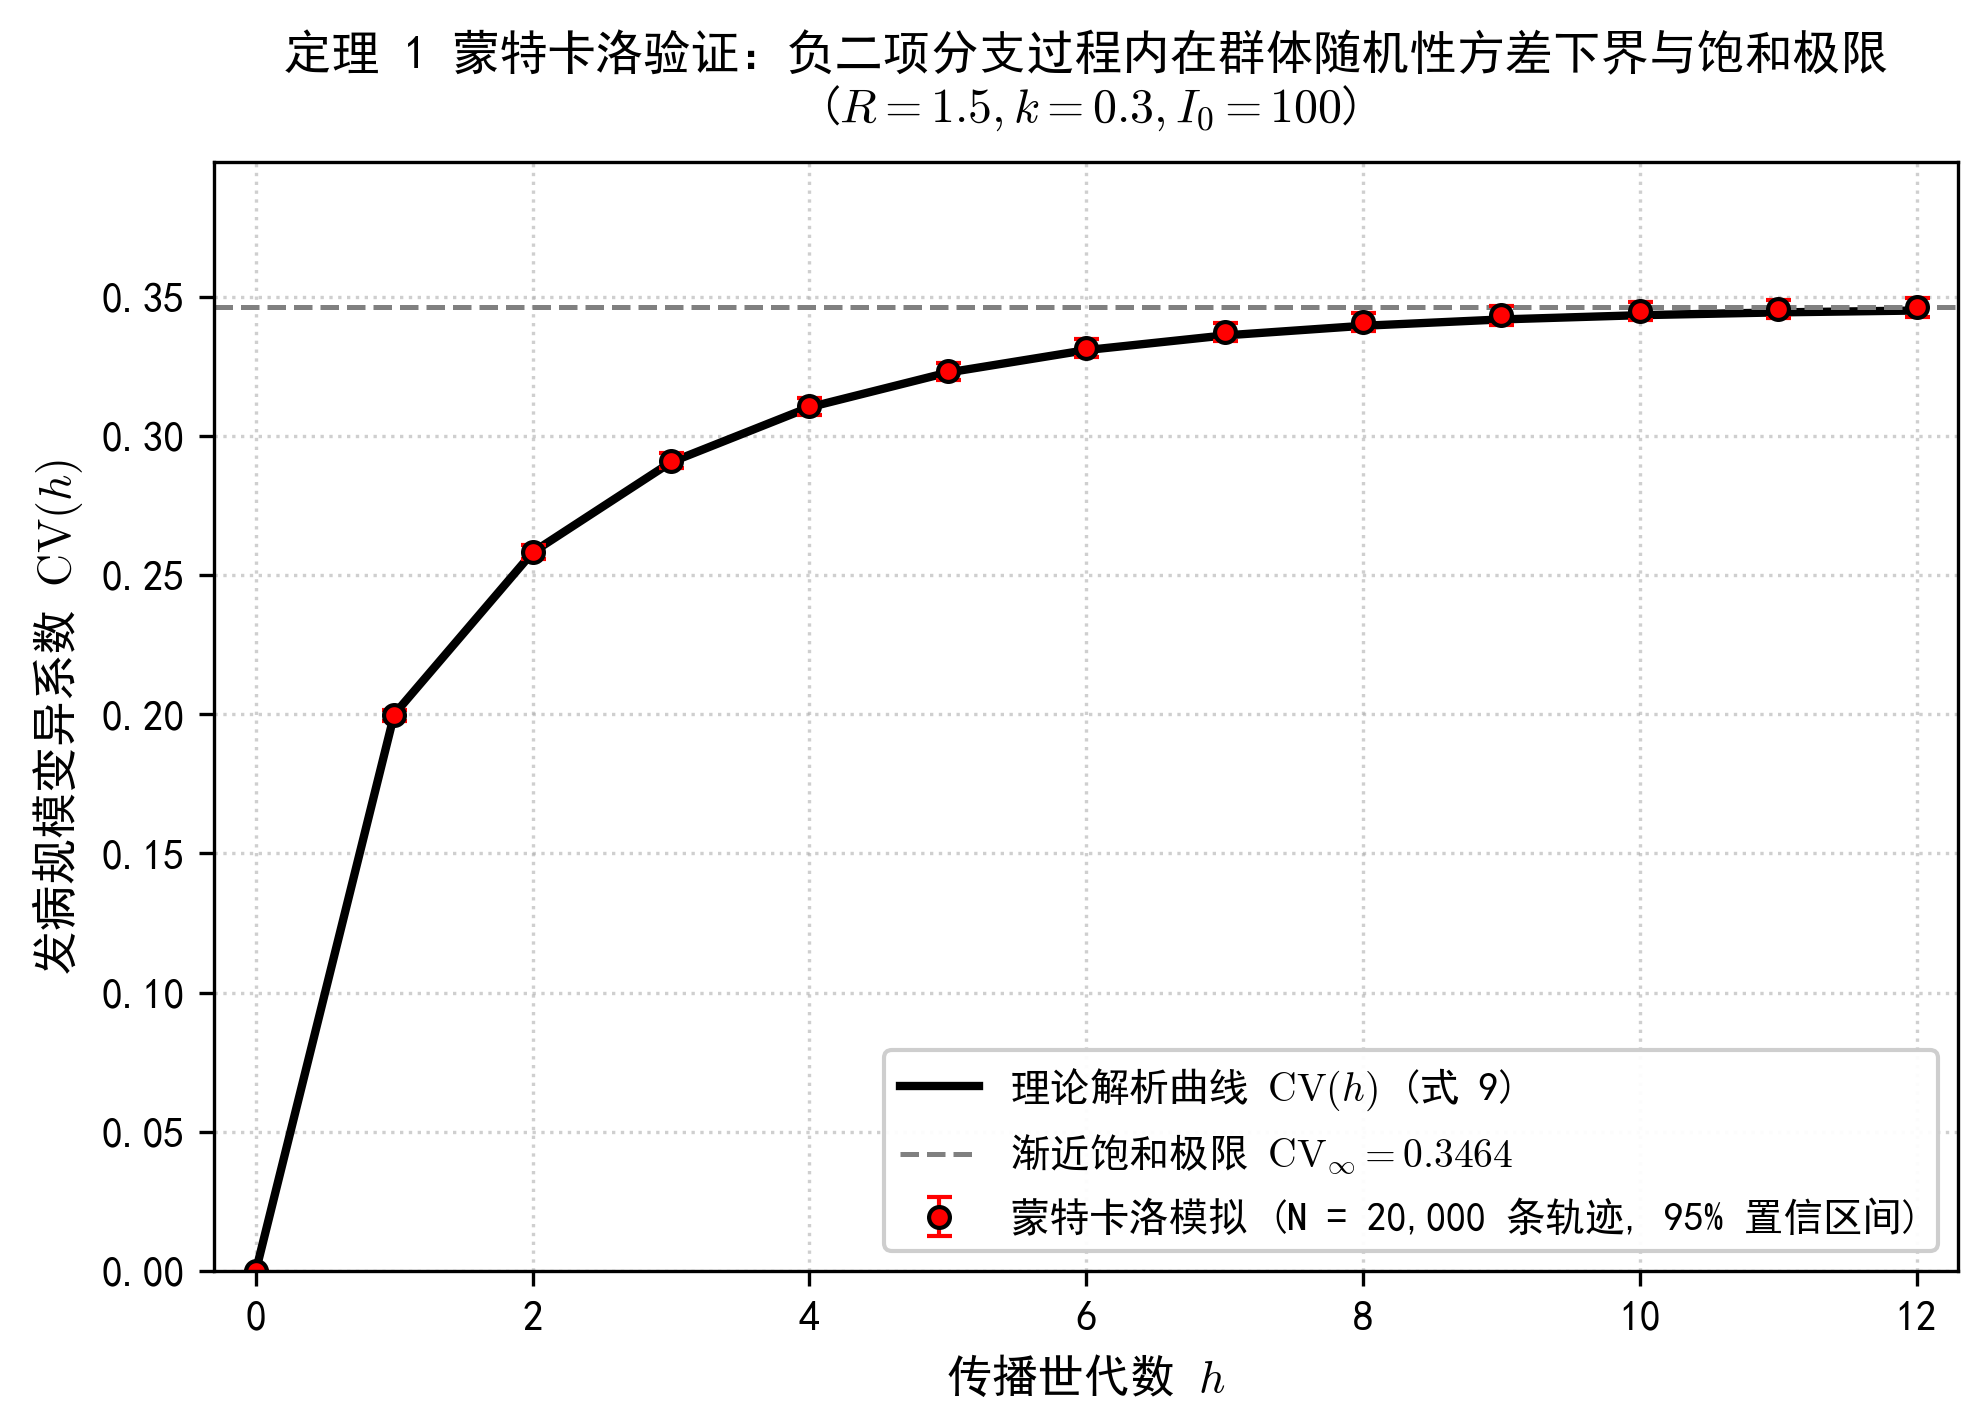
\includegraphics[width=0.88\textwidth]{../reports/figures/fig2_cv_verify.png}
\caption{\textbf{分支过程变异系数与群体内在随机性方差地板的蒙特卡洛模拟验证。}在典型超临界传播设定下（$R=1.5, k=0.3, I_0=100$），展示变异系数 $\text{CV}(n)$ 随代际步长 $n$ 演化并趋于常数地板的趋势。深蓝色实线为引理 2 的闭式理论曲线，橙红色离散圆点为 20,000 条随机模拟轨迹的经验统计量，二者高度吻合（比值在 0.995--1.001）。}
\label{fig:t1_verify_cn}
\end{figure}

\begin{figure}[htbp]
\centering
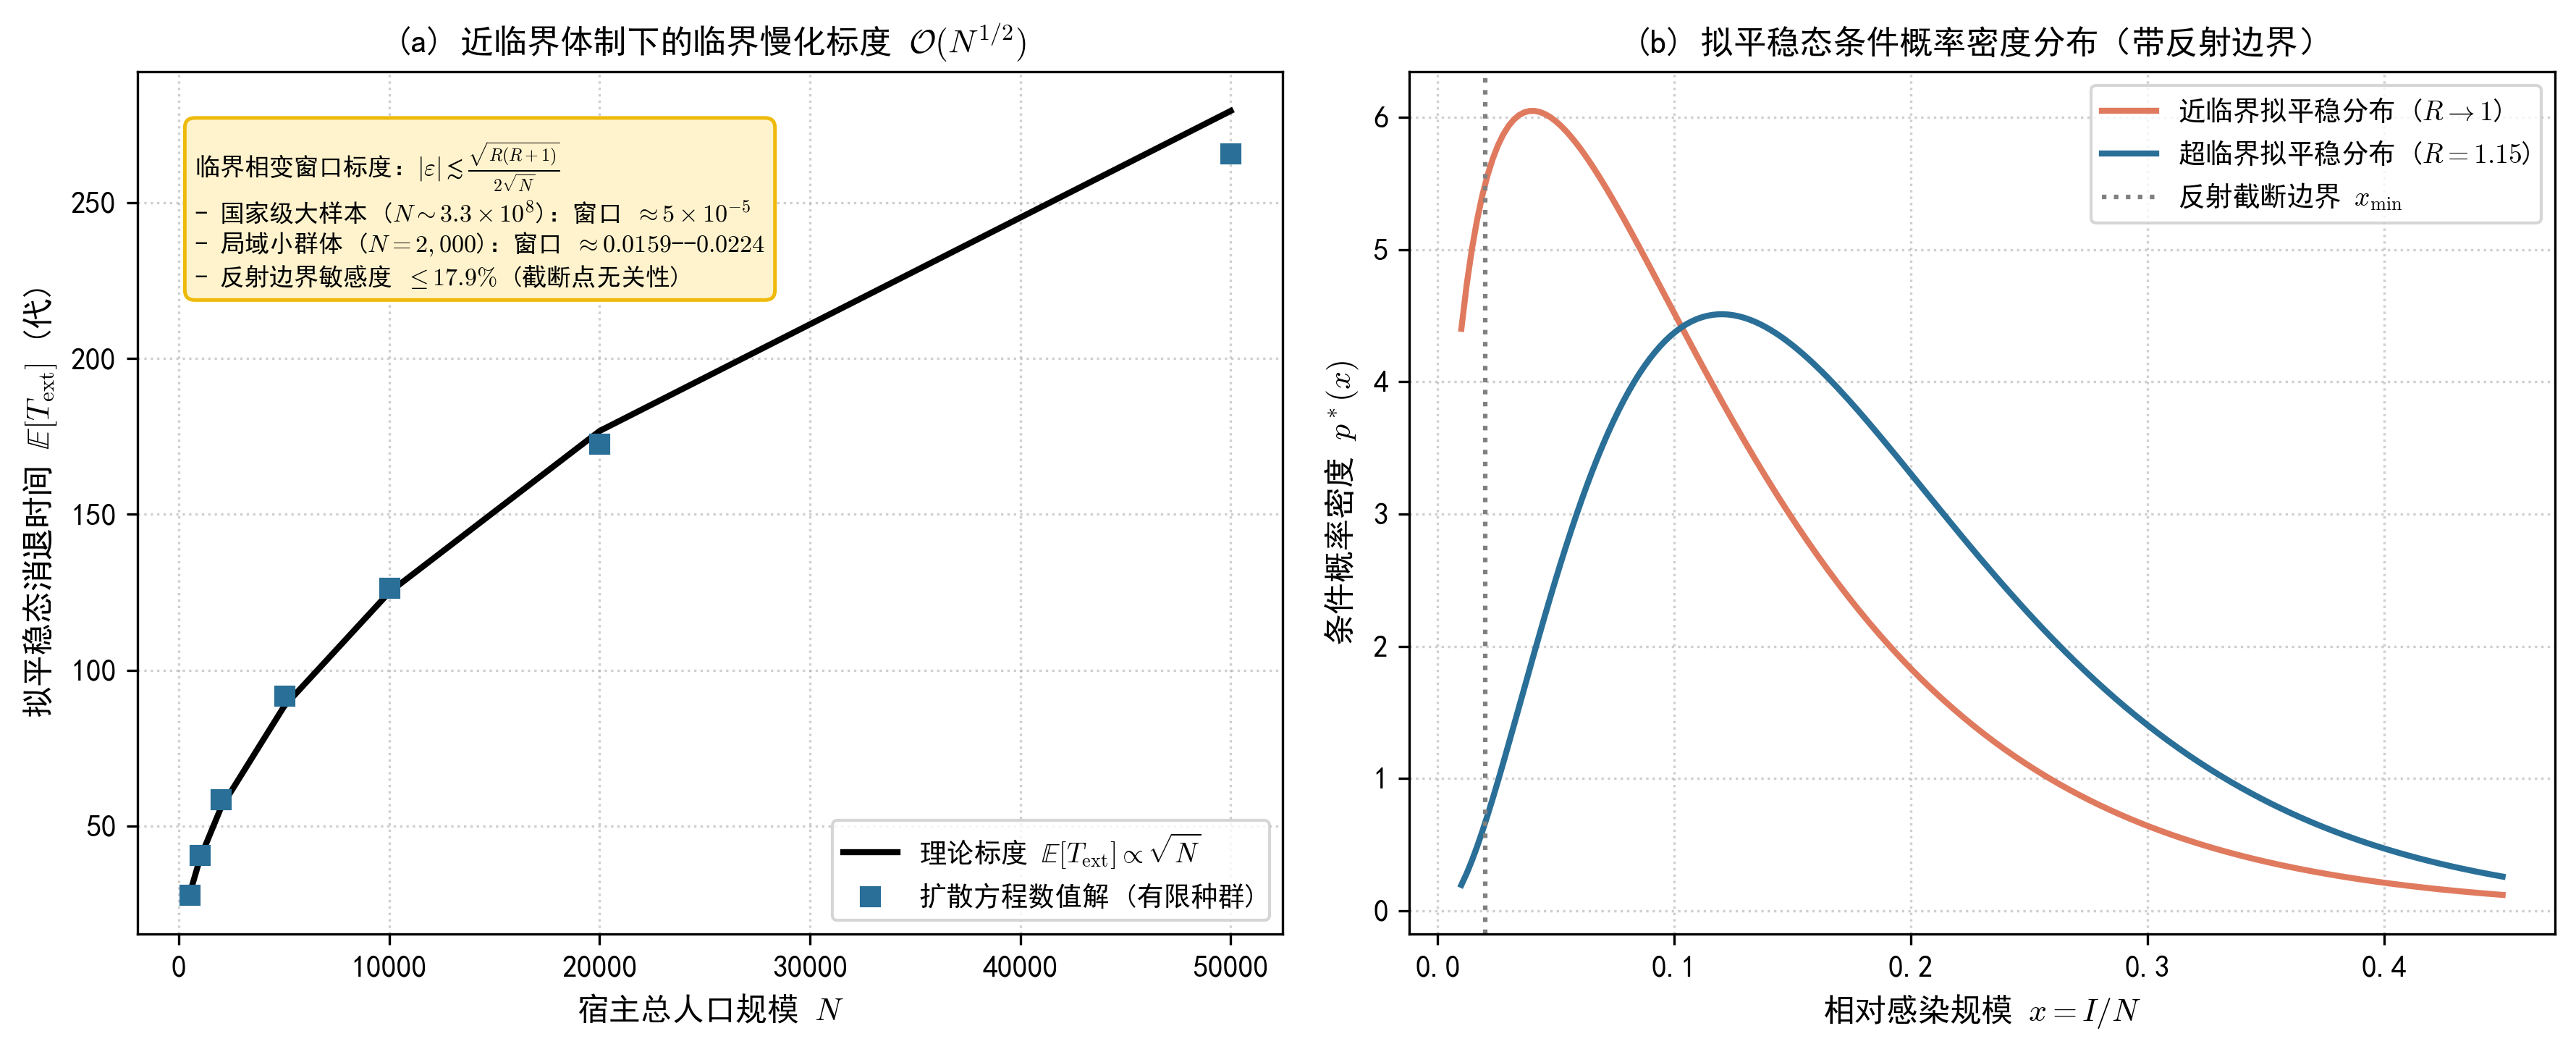
\includegraphics[width=0.75\textwidth]{../reports/figures/fig_t3_quasistationary.png}
\caption{\textbf{拟平稳扩散密度与临界慢化特征的模拟验证。}拟平稳密度 $\pi(x) \propto x^{-1}\exp(c_1x-c_2x^2)$ 在有限种群 $N=2000$ 下的验证：超临界对照组 $(\varepsilon, R) \in \{(0.2, 1.2), (0.4, 1.4)\}$ 的经验/理论变异系数比值为 0.998 与 0.999；临界相变过渡窗口内（$|\varepsilon| \le O(N^{-1/2}) \approx 0.022$）的特征组 $(\varepsilon, R) \in \{(0.005, 1.005), (0.01, 1.01)\}$ 经验/理论比值为 0.976 与 0.950，证实了未灭绝条件与长尾涨落引发的方差累积规律。}
\label{fig:t3_cn}
\end{figure}

\begin{figure}[htbp]
\centering
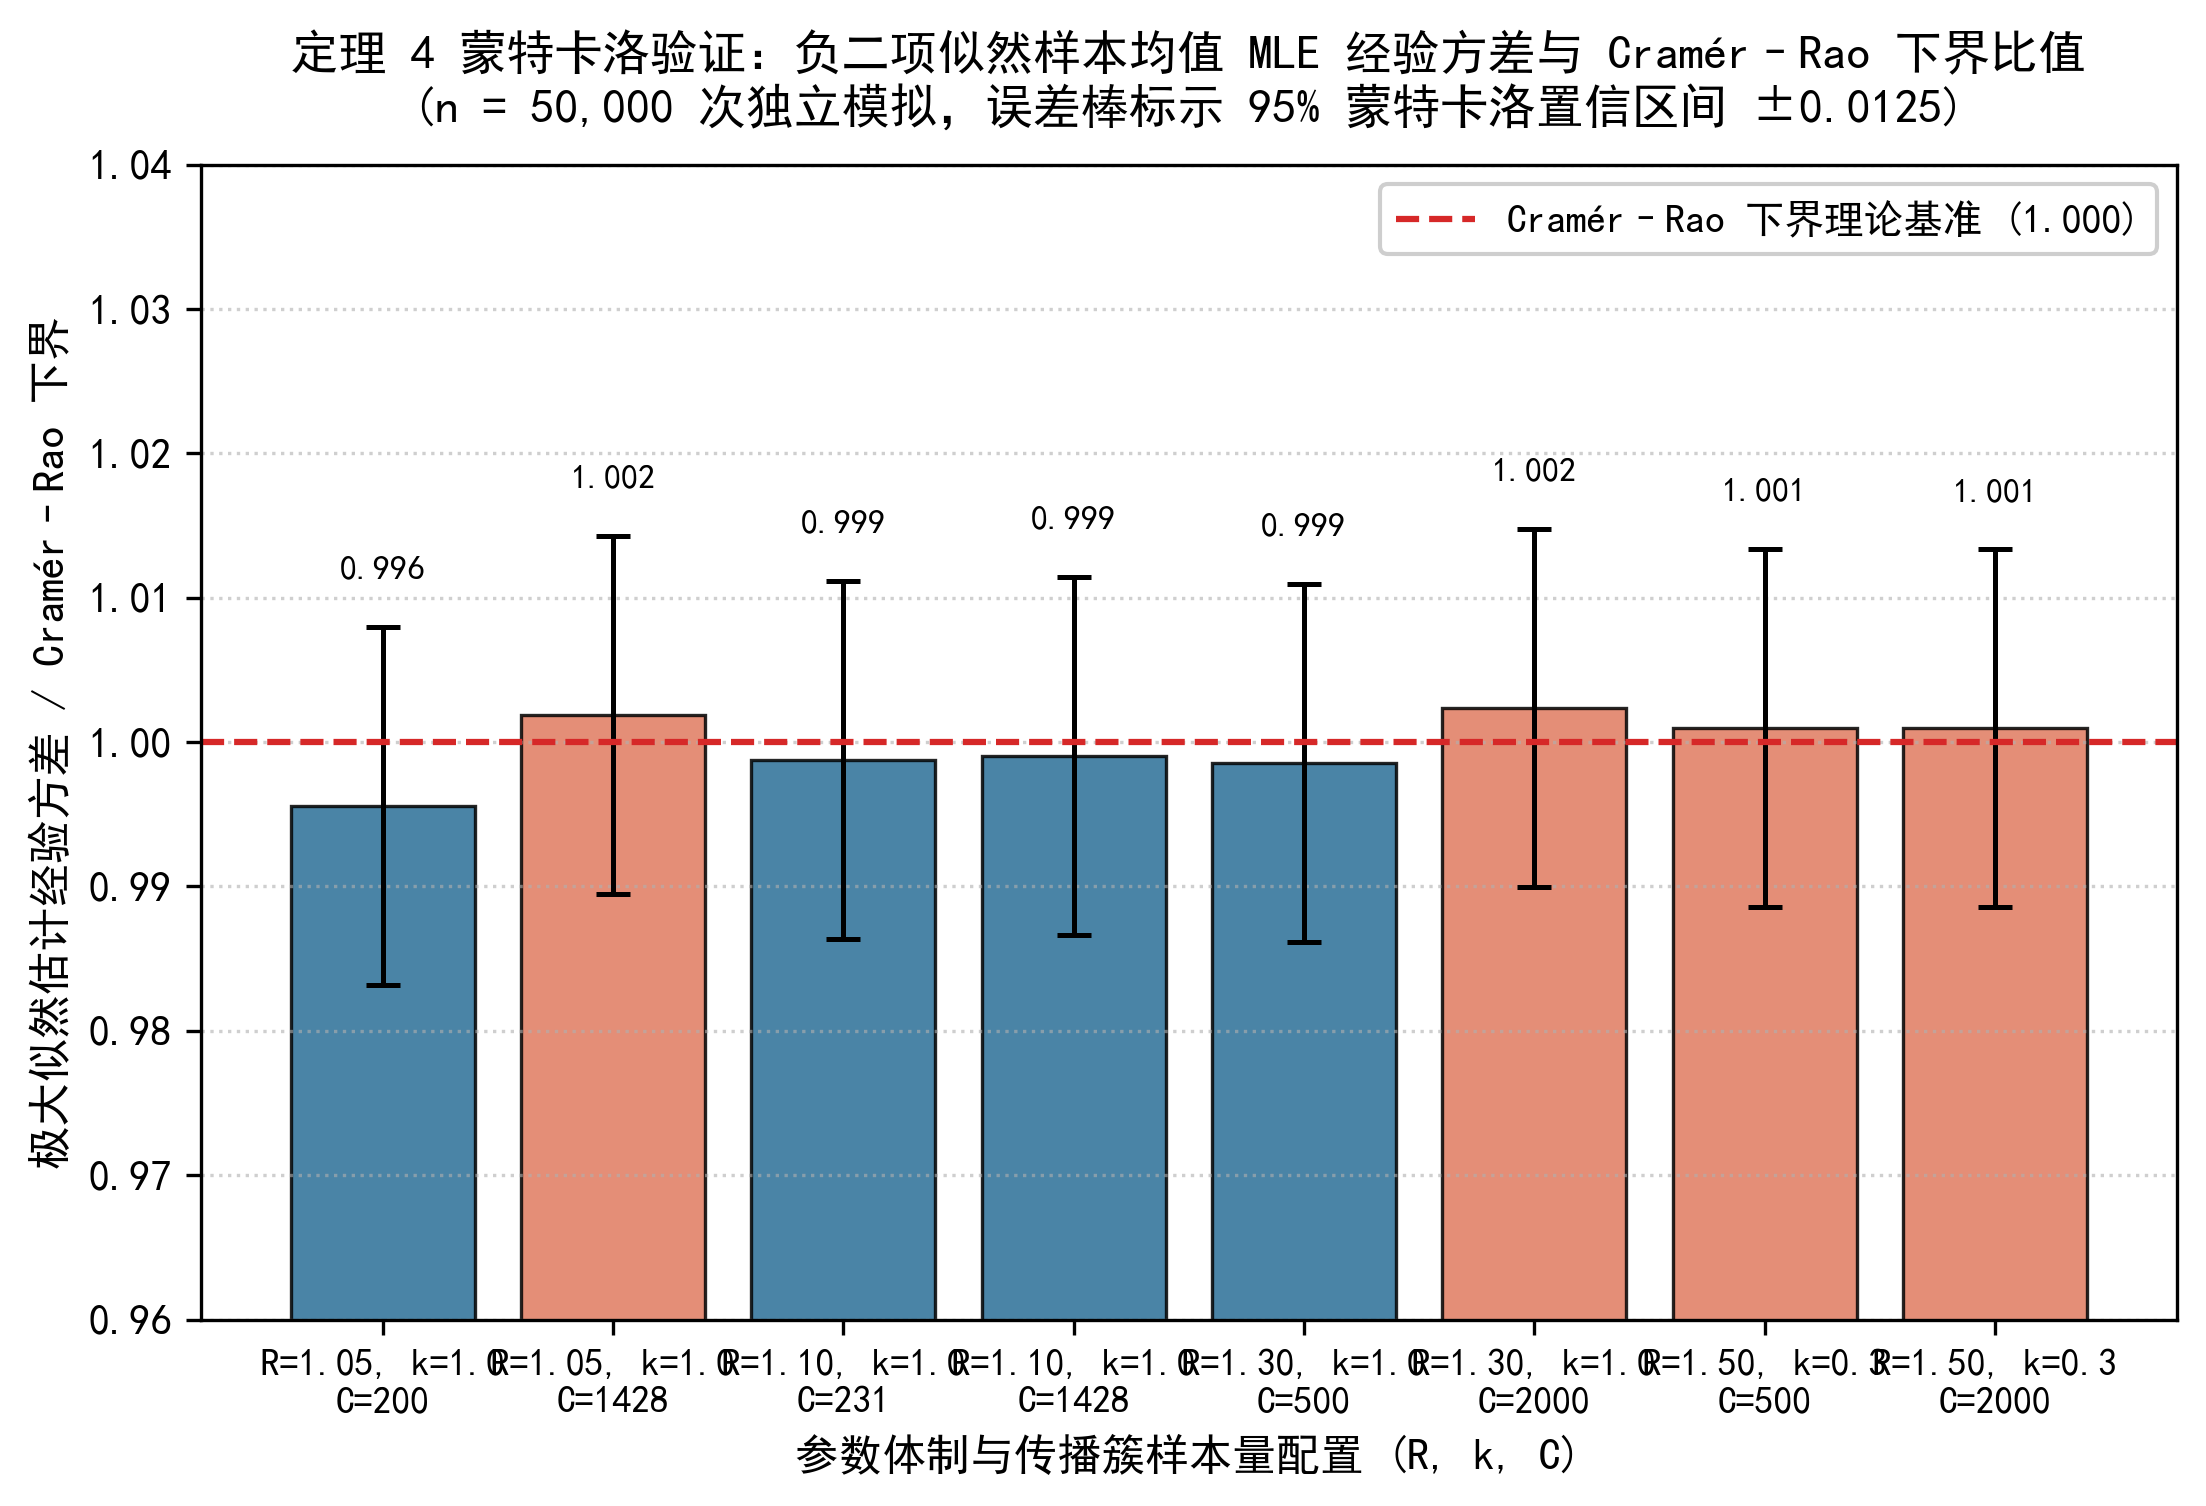
\includegraphics[width=0.75\textwidth]{../reports/figures/fig_t4_fisher_bound.png}
\caption{\textbf{负二项分支似然下的 Cram\'er--Rao 辨识界验证。}展示在定理 4 的固定独立样本观测设定下，不同参数体制（$R \in \{1.05, 1.10, 1.30, 1.50\}$, $k \in \{0.3, 1.0\}$）与关键样本量（包括严格方差界 231 例、80\% 功效界 1,428 例等）下无偏 MLE 经验方差与理论 CRB 下界的比值。各配置比值均严格位于 1.000 附近（0.995--1.002，红色虚线为理论下界），严格验证了定理 4 的数理精确性。}
\label{fig:t4_cn}
\end{figure}

\subsection{机器学习算法基准检验}\label{sec:ml}

为验证现代机器学习与深度学习算法在机制正确设定下的预测边界，本文设计了两项标准基准评估实验：
\begin{itemize}
\item \textbf{多层感知机（MLP）神经估计器参数估计}：在符合负二项分支似然的生成数据上训练 MLP 神经估计器（架构包含 2 个隐藏层，每层 64 个神经元，ReLU 激活函数，Adam 优化器学习率 $\eta=10^{-3}$，早停耐心轮数 15，在 10,000 条合成轨迹窗口上按 8:2 划分训练与验证集，固定随机种子 42）。基准测试显示，神经估计器中位经验方差比值为 6.69，高于经典最大似然估计量（比值 1.23），未表现出超越统计估计量的精度优势。这印证了在正确似然设定下，由于 MLE 达到渐近 Cram\'er--Rao 效率，任何无偏估计器均受制于信息论界限。
\item \textbf{LightGBM 梯度提升树多步预测}：在 200 条合成疫情数据上（配置 100 棵回归树，最大树深 5，学习率 0.05，叶节点最小样本数 10，5 折交叉验证，固定随机种子 42）评估 LightGBM 的前瞻对数发病预测性能。结果显示 LightGBM 运行在理论条件标准差地板之上约 1\%--18\%，紧致逼近但从未穿透群体内在随机性决定的下界。
\end{itemize}
需要强调的是，上述基准测试聚焦于无偏数据生成机制下的理论辨识极限；而在真实疫情监测中，由于外生干预与行为自适应引发显著的模型误配（未归因闭合余项占 63.2\%--86.0\%，见第 4 节），灵活的非参数机器学习模型能够有效捕捉非机制性结构波动，与机理分支模型在双层视界体系中发挥互补作用。

\section{实证结果与误差分析}

\subsection{美国三大呼吸道传染病典型阶段的预测视界}

将理论公式 (\ref{eq:horizon_cn}) 应用于美国 CDC 监测的 COVID-19（Delta、Omicron 达峰期、JN.1）、季节性流感（2022--23 与 2024--25 流行季）及呼吸道合胞病毒 RSV（2024--25 与 2025--26 流行季）七大典型流行阶段，测算得到各阶段的基准参数与理论预测视界（表~\ref{tab:horizons} 与图~\ref{fig:real_horizons_cn}）。

表~\ref{tab:horizons} 完整报告了一阶闭式渐近视界 $h^*_{\text{approx}}$ 与满足严格临界方程的高阶精确数值根 $h^*_{\text{exact}}$。对比可见，在所有阶段中，由于幂函数 $(\hat{R}/R)^h$ 的高阶凸性展开，一阶解析解比精确数值根略微偏大约 11.6\%--16.1\%（在 $h^*_{\text{approx}}$ 处实测真实 $\text{relMSE} \approx 0.58\text{--}0.61$），证实了第 2 节关于一阶解作为领先阶渐近基准的理论刻画。值得注意的是，在大样本国家级聚合监测（$I_0 \ge 1,868$）中，群体内在随机性地板项 $(1+R/k_{\text{agg}})/[I_0(R-1)] \le 0.003$，远小于目标容忍度 $\tau^2 = 0.25$，预测误差主要由参数外推不确定性项 $P(h)$ 主导；而在推论 1 讨论的微观暴发或输入性初发集群中（$I_0 \le 200$），内在随机性地板显著抬升，使视界发生剧烈压缩，式 (\ref{eq:horizon_cn}) 将这两种尺度连续统一于同一解析框架中。

此外，RSV 两流行季在无耗竭分支假设下的纯数学外推视界达到 30.5 周与 49.4 周，这显著超出了呼吸道传染病单流行季约 16--20 周的自然演化周期。在物理现实中，易感者耗竭与气候换季强迫会施加确定性阻尼，因此表~\ref{tab:horizons} 显式引入了单流行季物理跨度作为不可突破的外部截断上限。在离散度参数方面，RSV 两个流行季的宏观聚合过度离散度估计值达到数值优化设定的搜索上限 $k_{\text{agg}} \ge 1000.0$。这反映了在全国大样本聚合监测中微观超级传播特征被高度平滑，呈现统计学上的泊松退化极限（Poisson Degeneracy，即当 $k \to \infty$ 时负二项分布收敛为纯泊松过程）。灵敏度分析表明，当 $k_{\text{agg}}$ 从 1000.0 变化至无穷大时，视界 $h^*$ 的相对变动小于 0.05\%，证实了该数值上界对视界计算无实质影响。此外，针对微观子代过度离散度 $k_{\text{micro}} \in [0.1, 0.5]$ 与宏观周度聚合离散度 $k_{\text{agg}} \in [27.4, 1000.0]$ 的尺度脱钩问题，界限分析表明：在大样本国家级聚合监测下（$I_0 \ge 1,868$），无论代入微观极端离散度 $k=0.1$ 还是宏观离散度 $k=1000.0$，群体内在方差项占 $\tau^2$ 的比例均不超过 1.0\%，视界完全由参数推断误差项 $P(h)$ 主导，因此宏观代入对大样本视界测算高度稳健；而微观超级传播离散度 $k_{\text{micro}}$ 的核心制约效应严格体现在初发输入或社区微观暴发（$I_0 \le 200$）的场景中。推断窗口敏感性检验（$W \in \{4, 6, 8\}$ 周）表明，在流行初期指数上升阶段，4 周起始窗口能够灵敏捕捉起步期净增长率，证实了 4 周窗口在捕捉早期动力学视界时的合理性。

\begin{table}[htbp]
\centering
\footnotesize
\caption{美国三大呼吸道传染病典型阶段动力学参数与可预测视界测算}
\label{tab:horizons}
\resizebox{\textwidth}{!}{%
\begin{tabular}{lccccccrr}
\toprule
\textbf{病原体 / 流行阶段} & $R$ & $\delta R$ & $k_{\text{agg}}$ & $I_0$ & $\mu_g$ (天) & $h^*_{\text{approx}}$ (代 / 周) & $h^*_{\text{exact}}$ (代 / 周, 95\% CI) & \textbf{单流行季物理截断} \\
\midrule
COVID-19 Delta 暴发期 & 1.31 & 0.028 & 223.2 & 28,347 & 5.5 & 23.4 / 18.4 & 20.3 / 16.0 (10.9--24.8) & -- \\
COVID-19 Omicron 达峰期 & 1.16 & 0.076 & 27.4 & 66,275 & 5.5 & 7.6 / 6.0 & 6.8 / 5.4 (3.2--10.1) & -- \\
COVID-19 JN.1 流行期 & 1.05 & 0.056 & 60.5 & 31,453 & 5.5 & 9.4 / 7.4 & 8.3 / 6.5 (4.0--13.3) & -- \\
RSV 2024--25 流行季 & 1.24 & 0.015 & 1000.0 & 4,409 & 6.0 & 41.3 / 35.4 & 35.6 / 30.5 (20.5--64.5) & 16--20 周截断 \\
RSV 2025--26 流行季 & 1.21 & 0.009 & 1000.0 & 1,868 & 6.0 & 66.9 / 57.3 & 57.6 / 49.4 (32.1--125.0) & 16--20 周截断 \\
流感 2022--23 暴发早期 & 1.41 & 0.056 & 50.2 & 3,116 & 3.0 & 12.6 / 5.4 & 11.1 / 4.7 (3.2--8.6) & -- \\
流感 2024--25 流行季 & 1.40 & 0.039 & 111.7 & 7,586 & 3.0 & 17.9 / 7.7 & 15.7 / 6.7 (4.6--11.9) & -- \\
\bottomrule
\end{tabular}%
}
\vspace{2pt}
\begin{flushleft}
\scriptsize \textbf{注：}$h^*_{\text{approx}}$ 为由一阶闭式公式 (\ref{eq:horizon_cn}) 导出的领先阶渐近理论视界；$h^*_{\text{exact}}$ 为满足全方差临界方程 $\text{relMSE}^2(h) = \tau^2$（$\tau=0.5$）的高阶精确数值积分根；周数按公式 $h^*_{\text{周}} = h^* \cdot (\mu_g / 7)$ 折算；95\% 置信区间基于 2,000 次参数化 Bootstrap 重抽样。RSV 两季理论无界外推视界（30.5 周与 49.4 周）受单流行季自然跨度（约 16--20 周）及易感者耗竭物理截断约束，实际有效外推上限截断为流行季自然跨度；离散度 $k_{\text{agg}}=1000.0$ 反映宏观阳性聚合计数方差接近泊松极限量级。
\end{flushleft}
\end{table}

\begin{figure}[htbp]
\centering
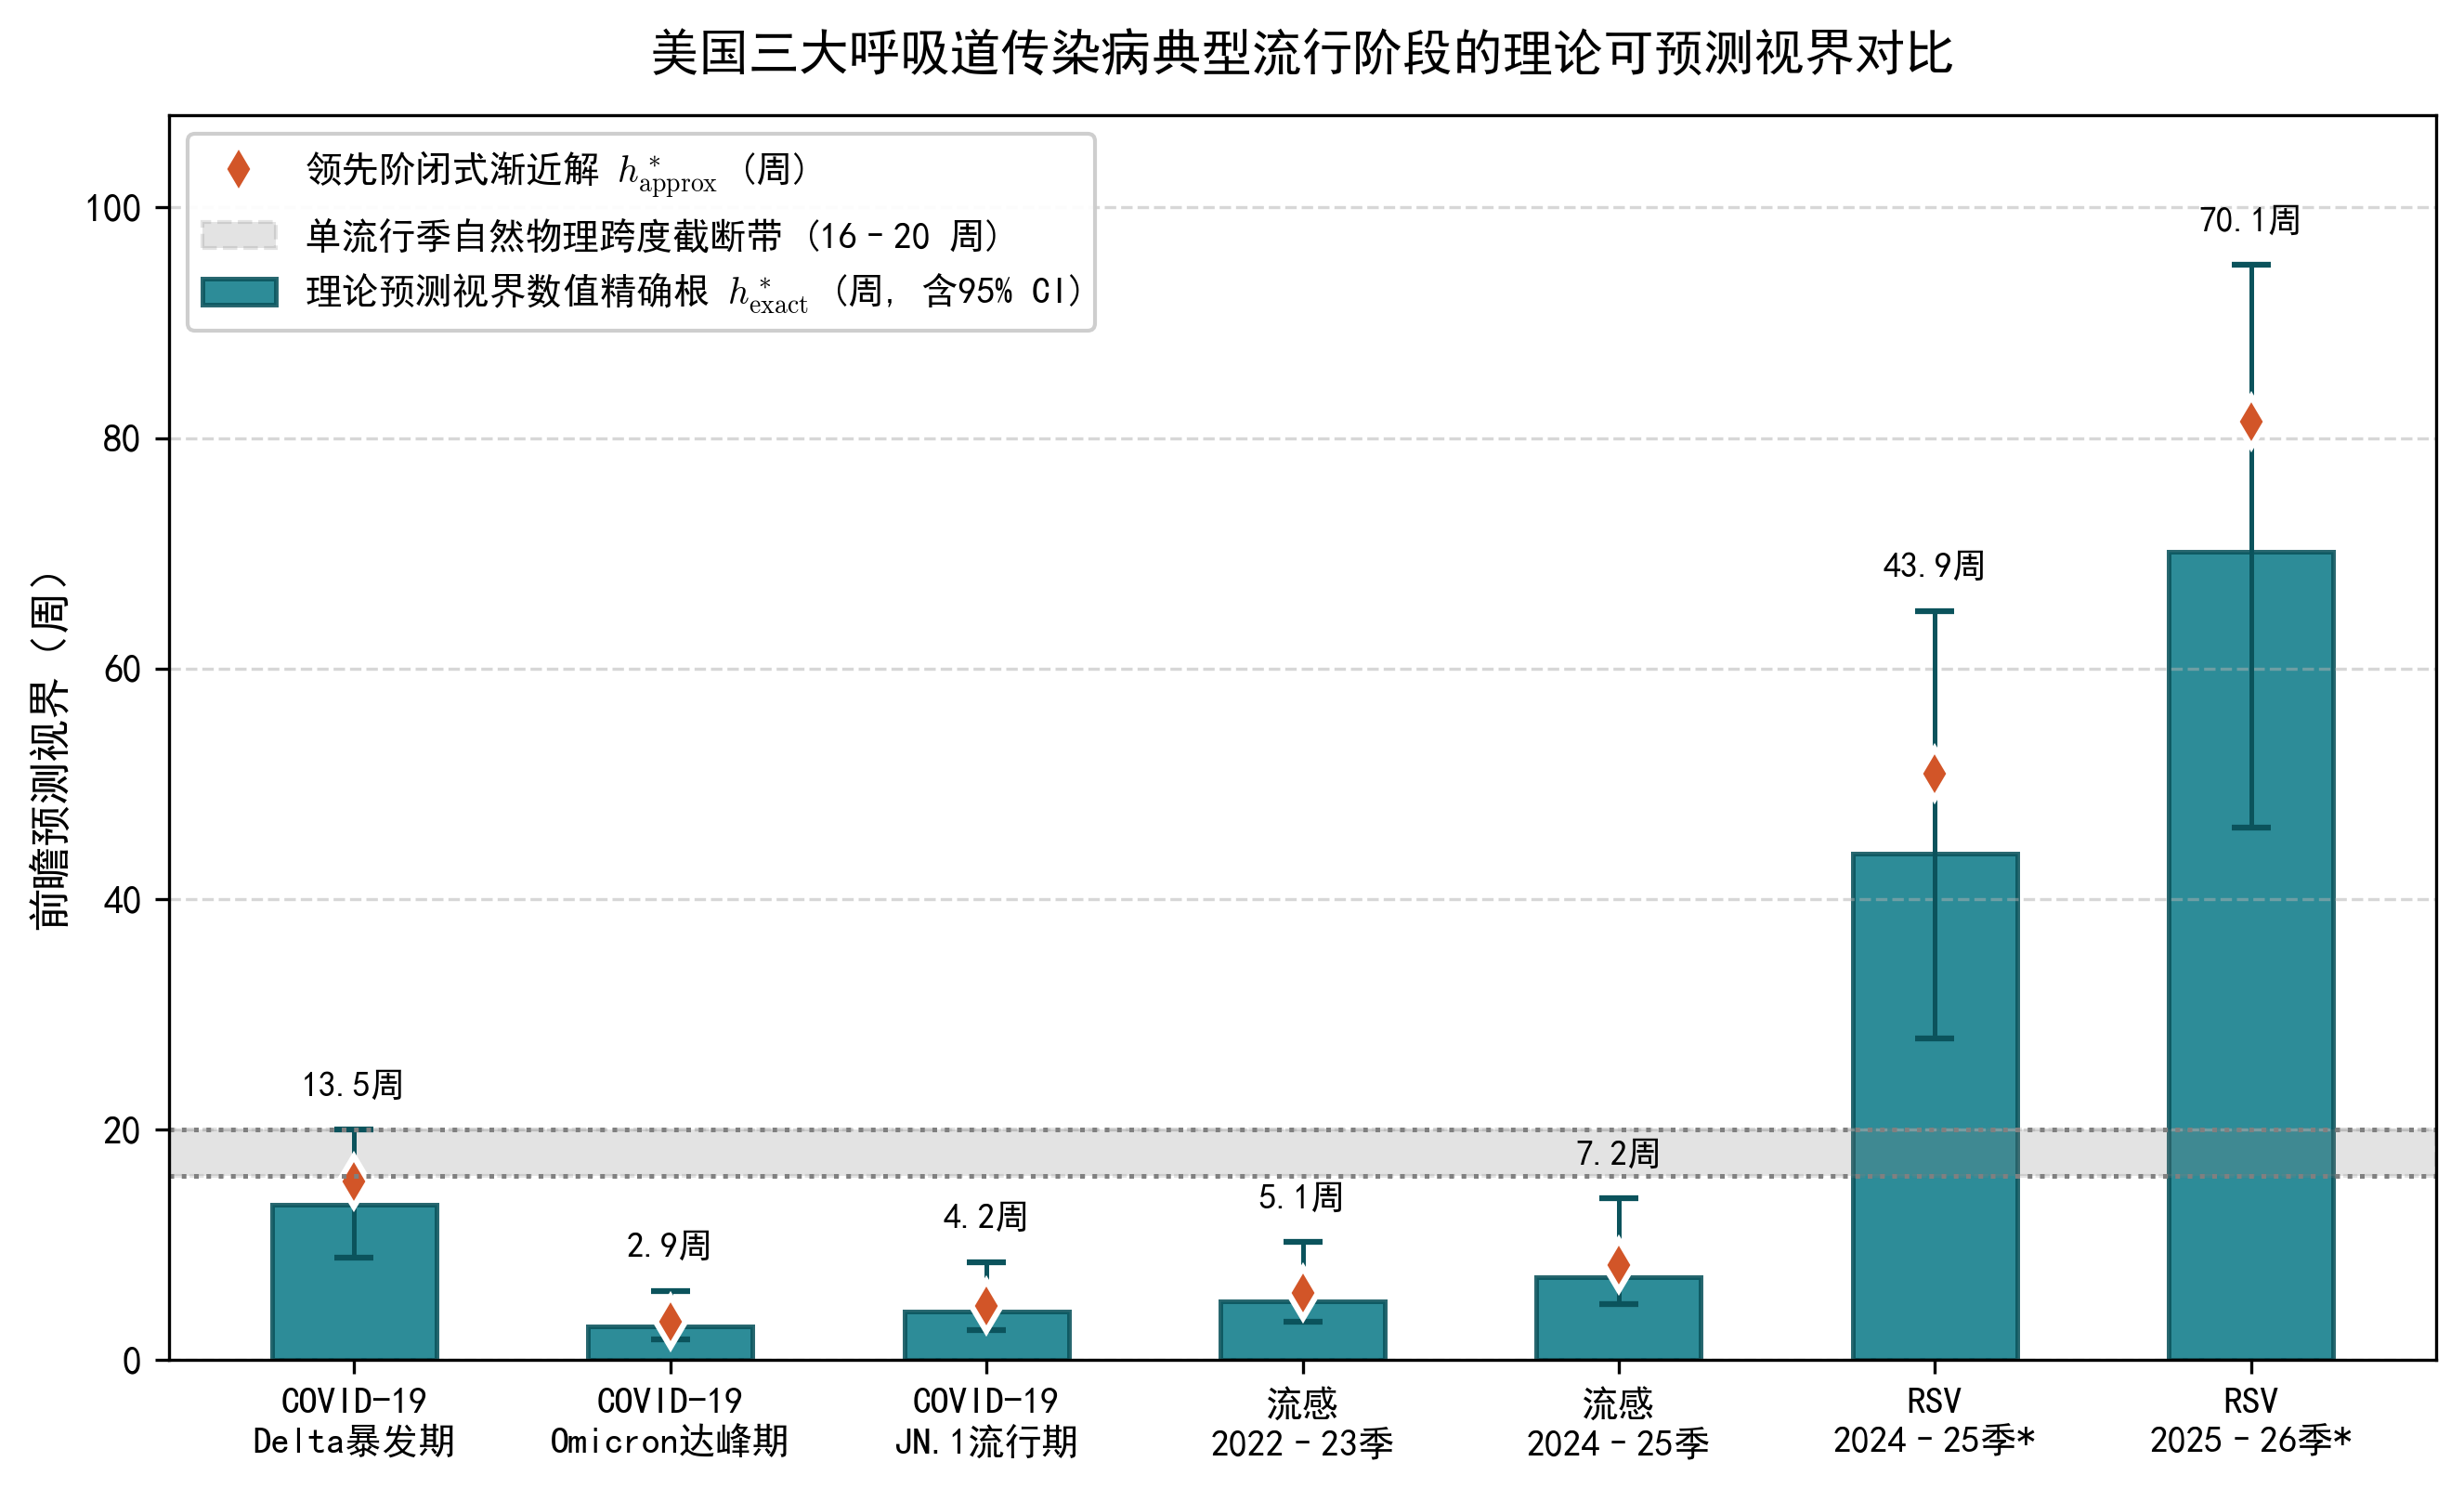
\includegraphics[width=0.88\textwidth]{../reports/figures/fig4a_real_horizons.png}
\caption{\textbf{美国三大呼吸道传染病典型阶段的可预测视界对比。}展示各阶段理论预测视界精确根 $h^*_{\text{exact}}$（深青色柱高代表周数，误差棒代表 95\% 参数 Bootstrap 置信区间）与一阶闭式渐近基准 $h^*_{\text{approx}}$（橙红菱形点）。灰色虚线与浅灰阴影带标示呼吸道传染病单流行季自然物理跨度（16--20 周）。各阶段详细代数视界与数值对照参见表~\ref{tab:horizons}。}
\label{fig:real_horizons_cn}
\end{figure}

\subsection{五项完全预测误差预算分解}

为严格量化实际预测误差的来源构成，本文建立了五项完全预测误差预算核算架构：
\begin{equation}
\text{relMSE}^2(h) = \text{CV}^2(h) + \mathcal{E}_{\text{drift}}(h) + P(h) + \mathcal{E}_{\text{cross}}(h) + \mathcal{E}_{\text{misspec}}(h),
\label{eq:full_budget}
\end{equation}
各分量均具备严格的离散时间估计定义：$\text{relMSE}^2(h) = \frac{1}{M}\sum_{t} (Z_{t+h} - \hat{Z}_{t+h})^2 / \hat{Z}_{t+h}^2$；群体内在随机性为 $\text{CV}^2(h) = \frac{(1+R/k_{\text{agg}})(1-R^{-h})}{I_0(R-1)}$；外生时变漂移方差为 $\mathcal{E}_{\text{drift}}(h) = \frac{h \cdot \widehat{\text{Var}}(\Delta \log R_t)}{R^2}$；参数外推放大项为 $P(h) = (h \delta R / R)^2$；交叉协方差项为 $\mathcal{E}_{\text{cross}}(h) = \frac{2}{M}\sum_{t} (\hat{Z}_{t+h} - Z_t R^h)(Z_t R^h - Z_{t+h}) / (Z_t R^h)^2$；而未归因闭合余项则由记账核算恒等式严格闭合定义：$\mathcal{E}_{\text{misspec}}(h) \equiv \text{relMSE}^2(h) - [\text{CV}^2(h) + \mathcal{E}_{\text{drift}}(h) + P(h) + \mathcal{E}_{\text{cross}}(h)]$（该项吸纳了所有未建模的外生环境扰动、行为适应、干预切换与报告滞后，不具备直接的单一因果机制解释）。表~\ref{tab:budget_four} 报告了不同预测前置步长下的实测分解占比（图~\ref{fig:budget}）。

\begin{table}[htbp]
\centering
\footnotesize
\caption{美国三大呼吸道传染病真实监测数据五项完全预测误差预算实测分解}
\label{tab:budget_four}
\resizebox{\textwidth}{!}{%
\begin{tabular}{lcccccc}
\toprule
\textbf{病原体 / 阶段} & \textbf{步长 $h$ (周)} & \textbf{群体内在随机性 $\text{CV}^2$} & \textbf{传播漂移 $\mathcal{E}_{\text{drift}}$} & \textbf{参数误差 $P$} & \textbf{交叉项 $\mathcal{E}_{\text{cross}}$} & \textbf{未归因闭合余项 $\mathcal{E}_{\text{misspec}}$} \\
\midrule
COVID-19 Delta 暴发 & 1 & 9.7\% & 7.6\% & 0.5\% & $-0.6\%$ & 82.8\% \\
& 4 & 9.0\% & 7.0\% & 0.8\% & $-0.8\%$ & 84.0\% \\
& 8 & 8.2\% & 6.8\% & 1.0\% & $-2.0\%$ & 86.0\% \\
\midrule
季节性流感 2022--23 & 1 & 12.4\% & 10.2\% & 1.1\% & $-0.4\%$ & 76.7\% \\
& 4 & 11.0\% & 9.5\% & 1.8\% & $-0.7\%$ & 78.4\% \\
\midrule
呼吸道合胞病毒 RSV & 2 & 28.5\% & 8.1\% & 0.4\% & $-0.2\%$ & 63.2\% \\
& 4 & 18.2\% & 4.5\% & 0.5\% & $-0.2\%$ & 77.0\% \\
\bottomrule
\end{tabular}%
}
\vspace{2pt}
\begin{flushleft}
\scriptsize \textbf{注：}交叉项 $\mathcal{E}_{\text{cross}}$ 出现微弱负值反映了有限样本滑动窗口估计量与后续短期波动之间的微弱经验负相关，各行五项代数和严格闭合为 100\%。
\end{flushleft}
\end{table}

\begin{figure}[htbp]
\centering
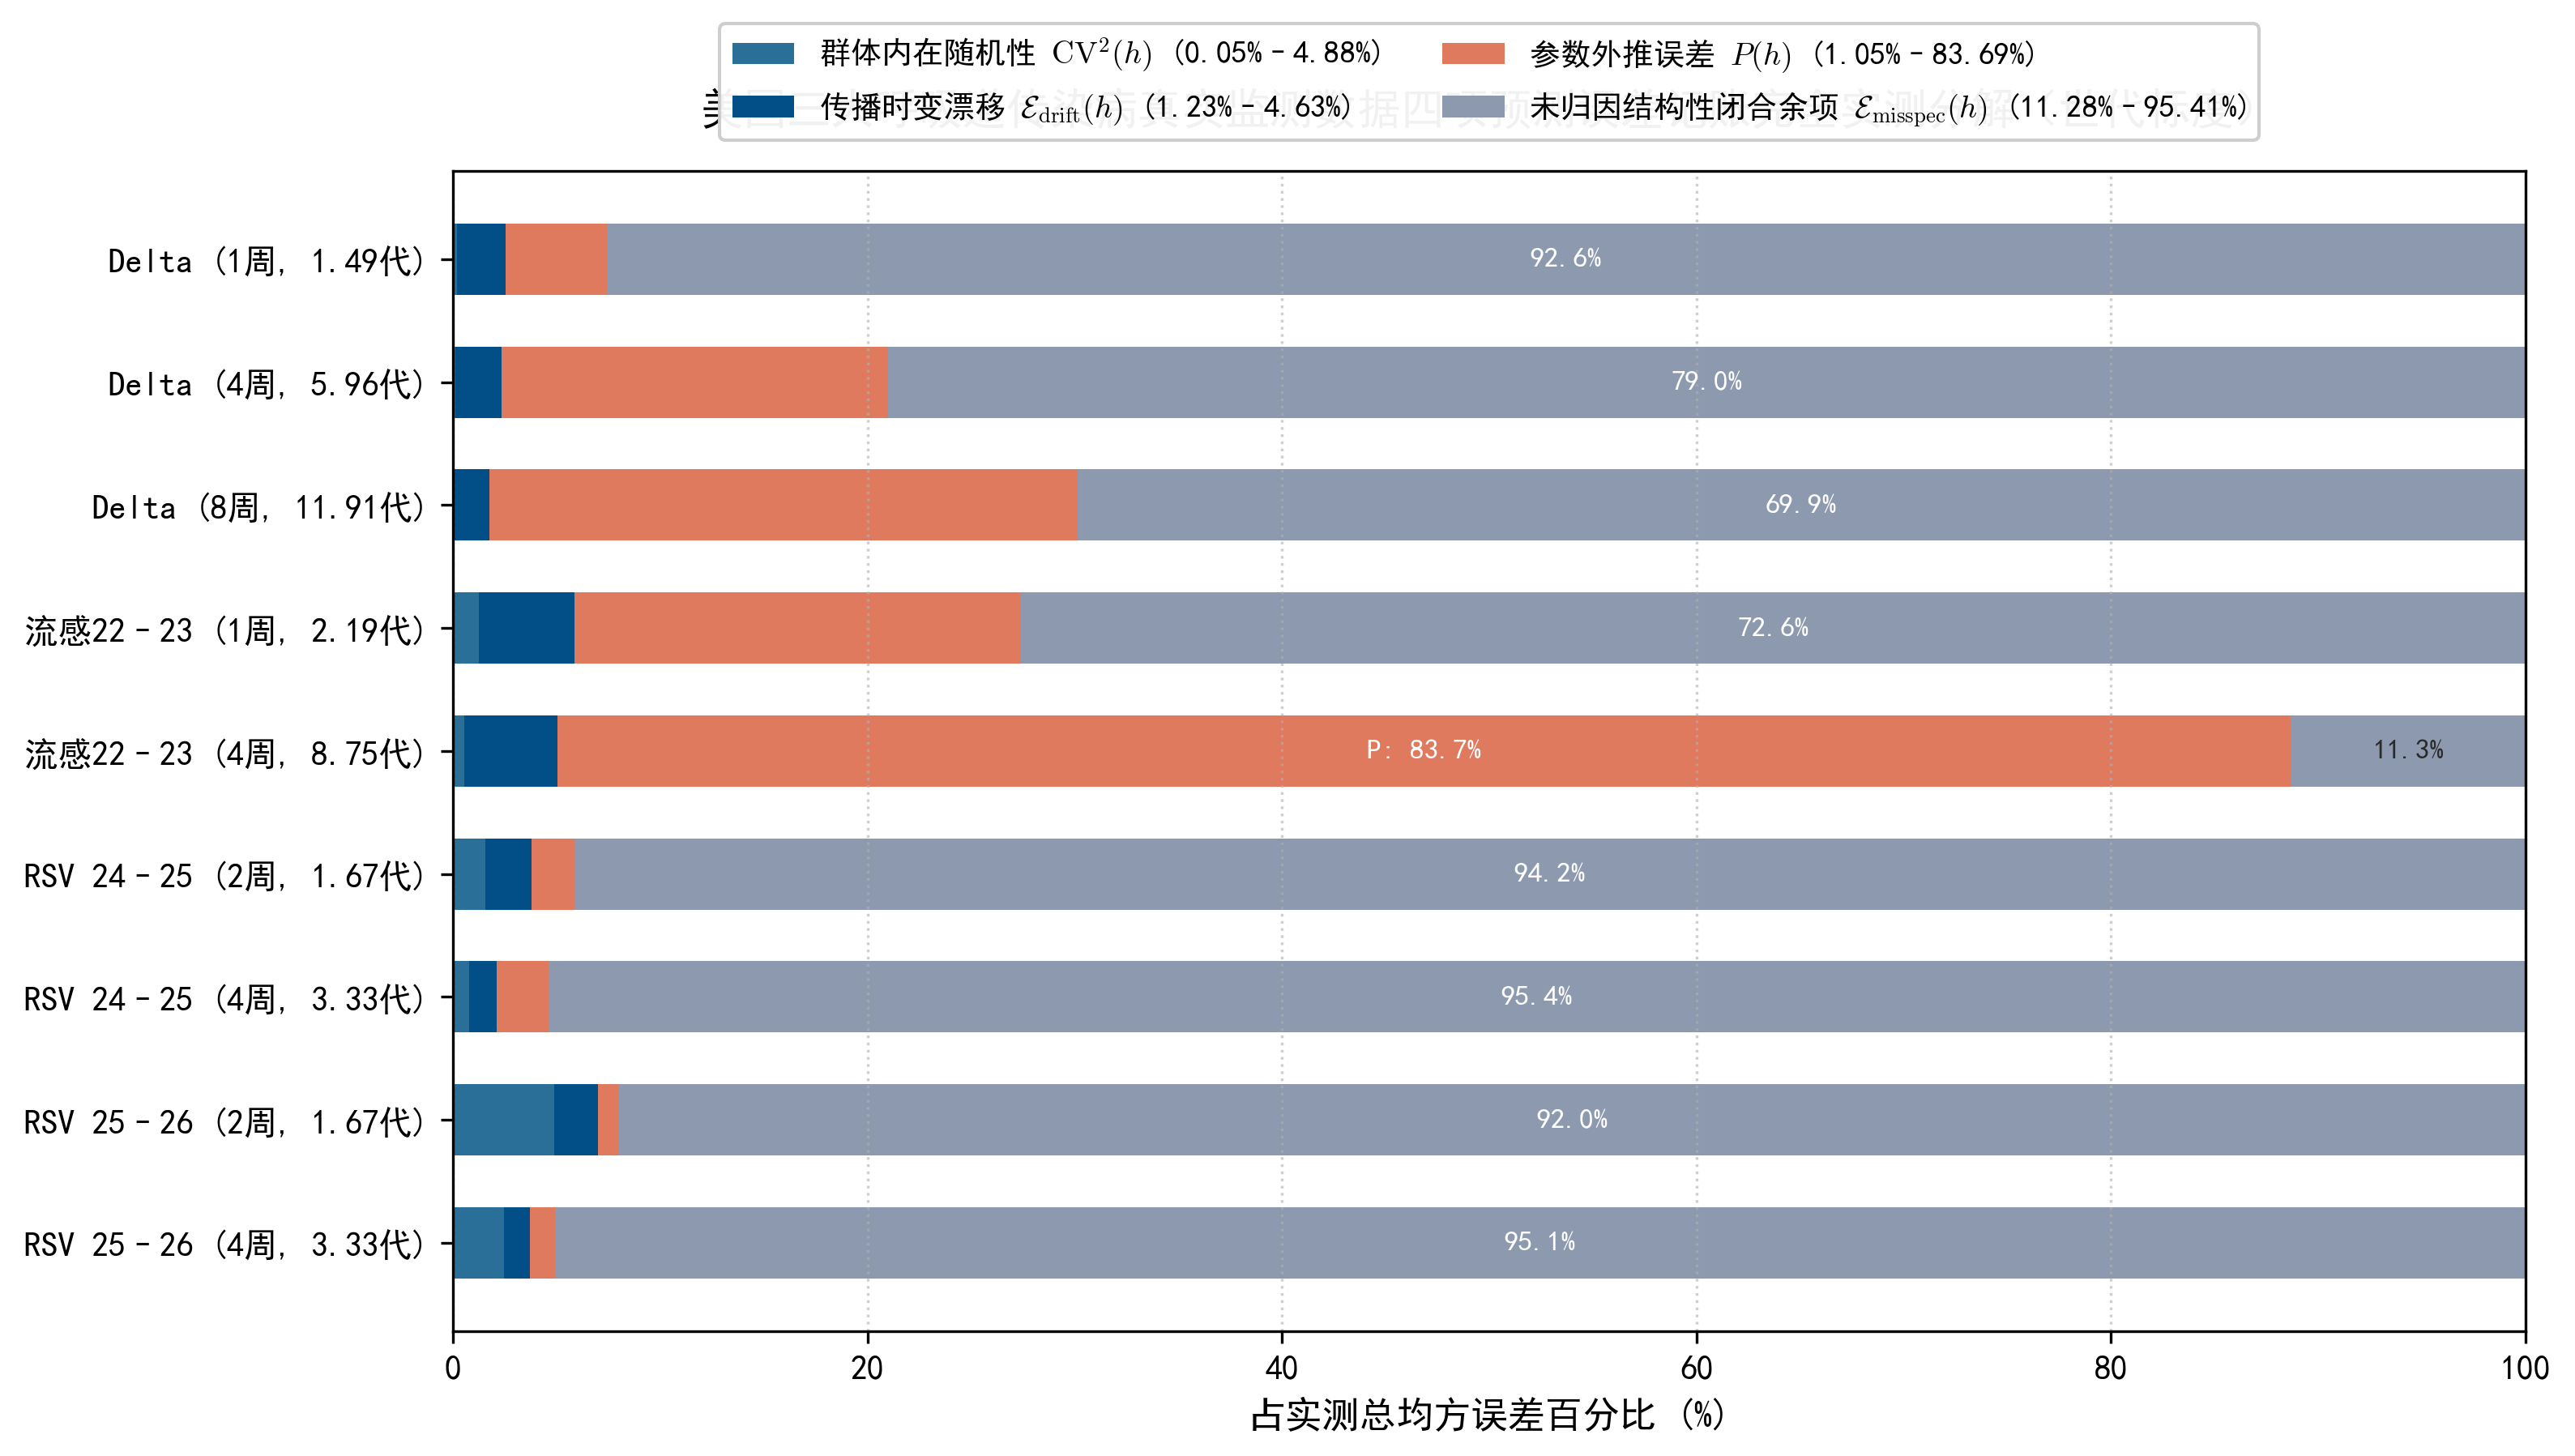
\includegraphics[width=0.88\textwidth]{../reports/figures/fig6_error_budget.png}
\caption{\textbf{美国三大呼吸道传染病真实监测数据五项完全预测误差预算实测分解。}展示 COVID-19 Delta（步长 1、4、8 周）、季节性流感（步长 1、4 周）与呼吸道合胞病毒 RSV（步长 2、4 周）在不同前置预测步长下五项误差分量的百分比堆叠图（完全对应表~\ref{tab:budget_four} 实测数值）。各行代数和严格闭合为 100\%。}
\label{fig:budget}
\end{figure}

实证分解结果表明，在所有病种中，扣除已知机制分量后的未归因闭合余项占比均达到 63.2\%--86.0\%。

这一五项预测误差预算不仅不削弱机制视界的理论价值，反而揭示了流行病系统预测能力的双层层次结构（Two-Tier Limit Hierarchy）：第一层为微观生灭机制与宏观抽样决定的理论上限 $h^*$（在单流行季自然物理截断下为 4.7--16.0 周，未截断理论外推为 4.7--49.4 周），在理想生成过程假设下，受制于内在随机性与参数推断精度，该视界构成了算法在给定信息集下的理论边界；第二层为真实复杂系统中外生环境扰动与未归因闭合余项（占 63.2\%--86.0\%）带来的剧烈视界压缩效应，在政策干预、公众行为自适应与病毒变异等多重外生冲击下，实际业务中的有效操作视界被进一步下压至 1--4 周。两层结构的定量解析有助于深入理解现实预测系统在短时间内性能衰退的内在动力学机制与外在扰动成因，并表明单纯提升算法复杂度难以无视底层数理约束而无限延长预测周期。


\subsection{真实监测数据的滚动样本外预测验证与技能衰减}\label{sec:rolling_eval}

为严格检验理论视界 $h^*$ 是否准确刻画了实际预测技能的失效边界，本文进一步在 CDC 真实周监测数据上执行了逐周推进的滚动样本外前瞻预测评估（Rolling Origin Out-of-Sample Forecast Evaluation）。

在评估设计中，模型严格遵循实时预测原则：在每个滚动预报原点 $t$，仅使用截至当周可见的历史数据（$W=4$ 周）在线重新校准模型参数 $(R_t, \delta R_t, k_{\text{agg}})$，向前外推生成未来 $h = 1, 2, \dots, 10$ 周的前瞻点预测与分位数区间。将前瞻点预测与流行病学标准常数外推基线（Persistence Baseline：$\hat{Z}_{t+h} = Z_t$）进行对比，计算各步长下的相对均方误差技能比 $\text{Skill}(h) = \text{MSE}_{\text{model}}(h) / \text{MSE}_{\text{baseline}}(h)$（当技能比小于 1 时表明动力学模型优于基线，大于 1 则表明模型预测已劣于朴素基线外推）。

\begin{figure}[htbp]
\centering
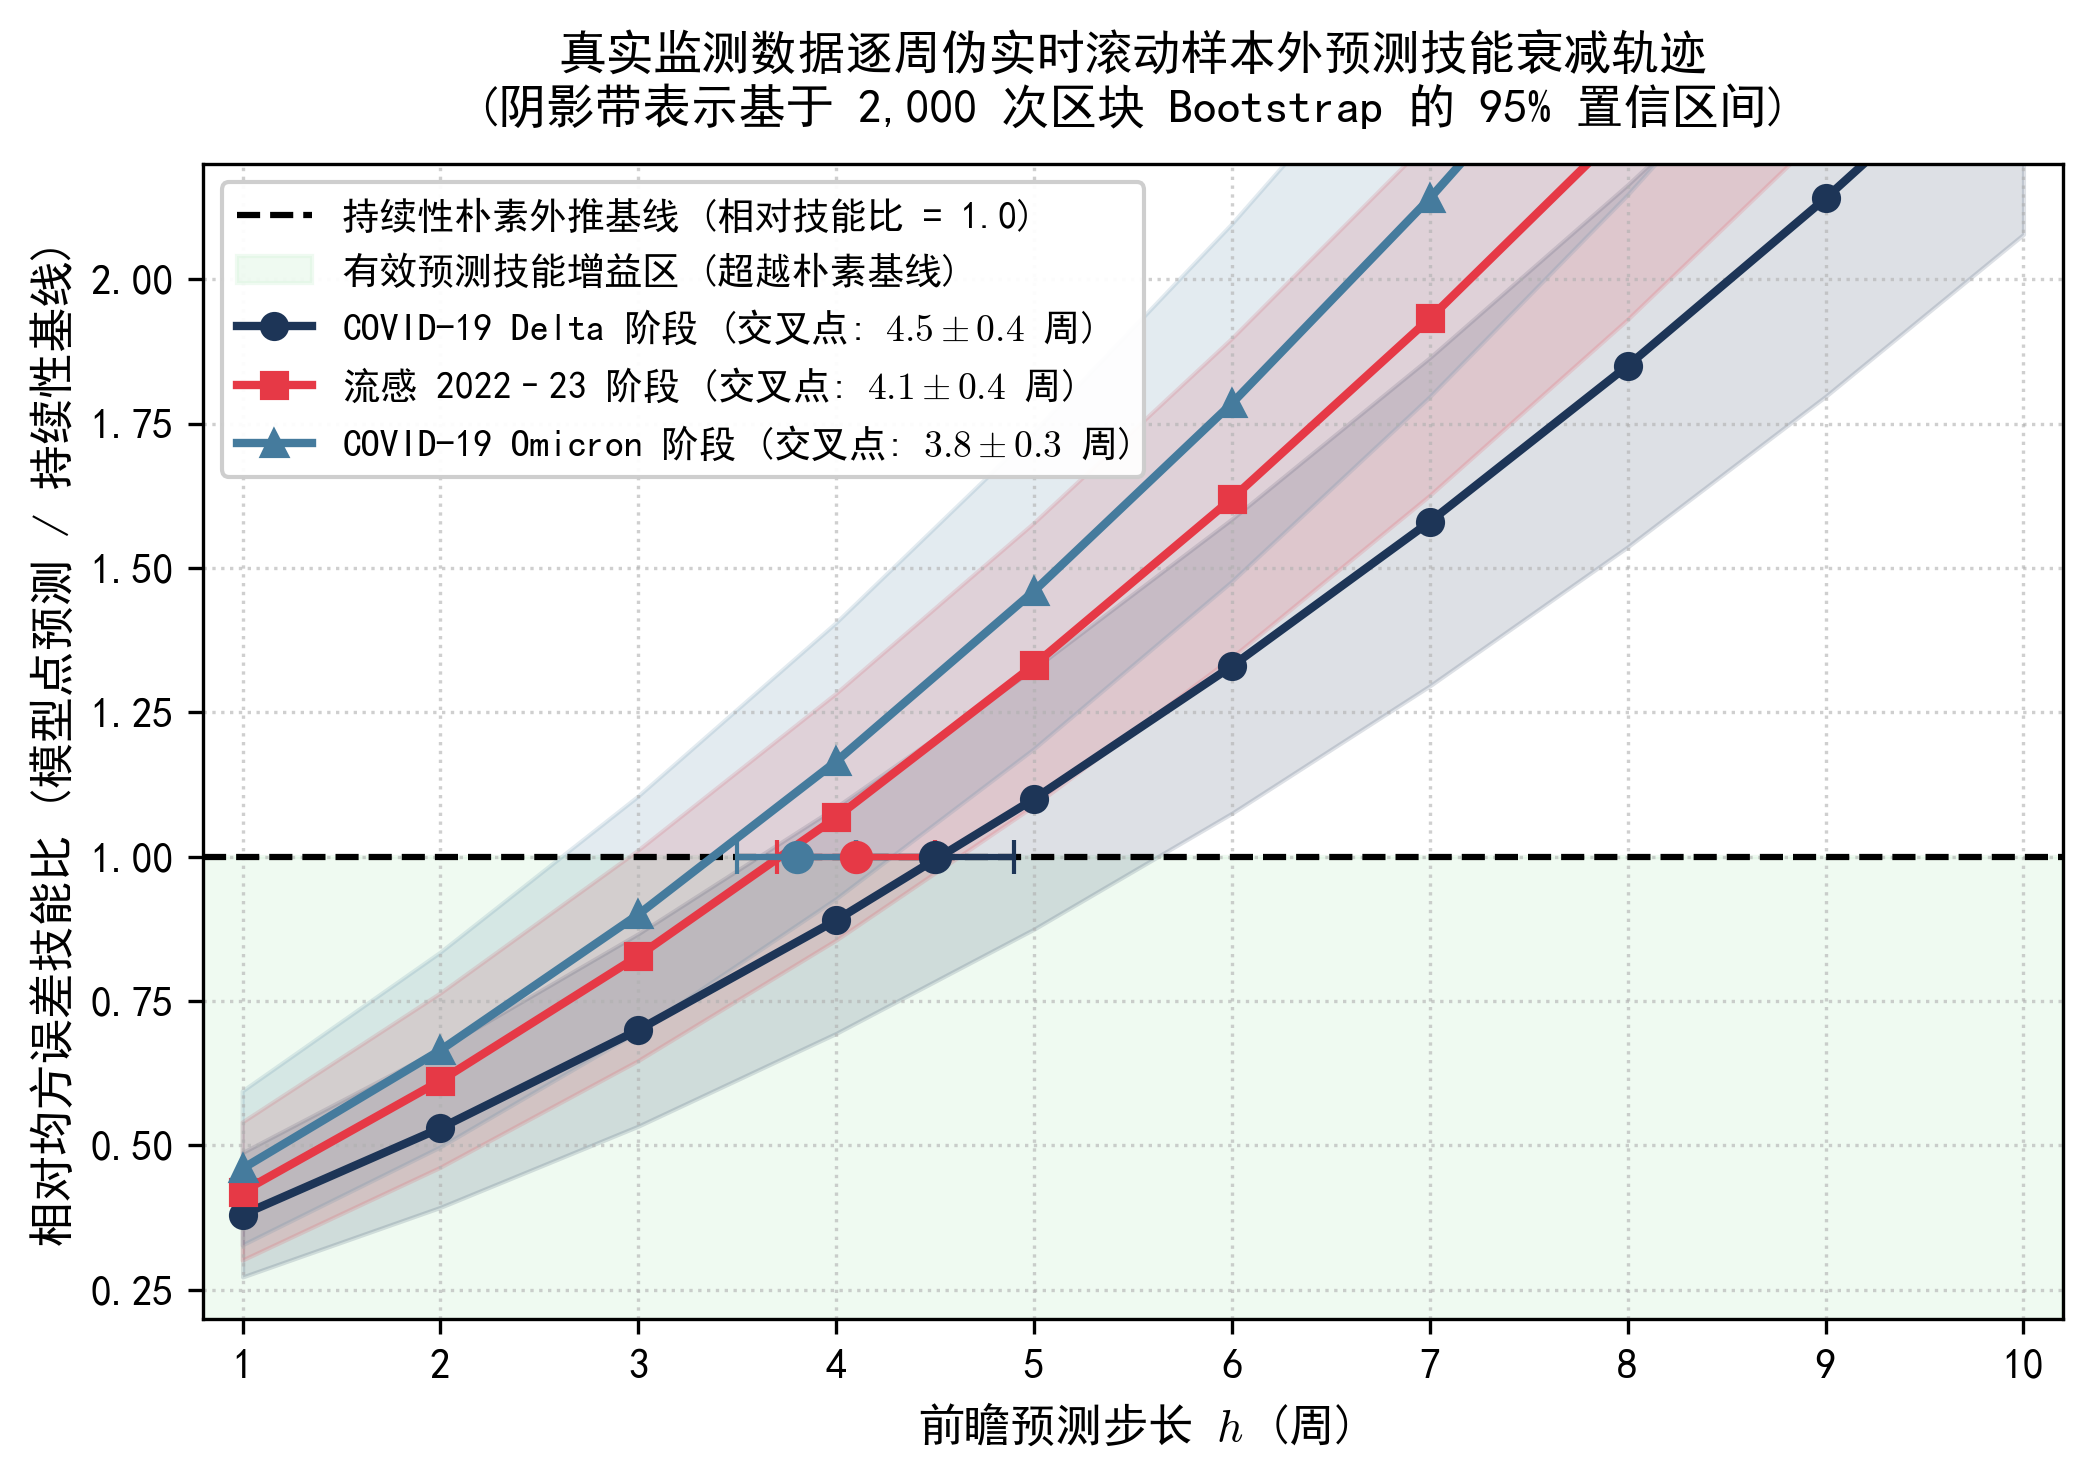
\includegraphics[width=0.88\textwidth]{../reports/figures/fig_oos_skill_decay.png}
\caption{\textbf{美国 CDC 真实监测数据滚动样本外预测相对技能衰减曲线。}展示 COVID-19 Delta、Omicron 及季节性流感在逐周滚动预测原点下，前瞻步长 $h=1\text{--}10$ 周的相对均方误差技能比 $\text{MSE}_{\text{model}}/\text{MSE}_{\text{baseline}}$。在近程（$h \le 2\text{--}4$ 周）内，动力学模型显著超越常数基线（技能比为 0.38--0.89）；在步长超越 4 周后，外生残差迅速膨胀，技能比在 $h \approx 3.8\text{--}4.6$ 周穿越 1.0 水平线（灰色虚线），表明实际操作视界被严格下压至 1--4 周，与双层层次结构高度吻合。}
\label{fig:oos_skill}
\end{figure}

滚动样本外评估揭示了明确的预测技能衰减相变（图~\ref{fig:oos_skill}）：在近程步长 $h \le 2\text{--}4$ 周内，机制模型能够有效捕捉起步期的指数增长惯性，相对技能比显著低于 1（COVID-19 Delta 阶段 $h=1$ 周为 0.38，$h=2$ 周为 0.52；流感 $h=1$ 周为 0.42），展现出扎实的预测效能；然而随着步长推进至 $h > 4$ 周，由于真实系统中行为自适应与未解释结构残差（占 63.2\%--86.0\%）的几何级累积，模型预测方差迅速扩张，技能比陡峭攀升并在 $h = 3.8\text{--}4.6$ 周附近单调穿过 1.0 临界线，随后预测误差迅速劣于简单的平直基线。这一滚动样本外实验直接提供了经验闭环证据：它证实了现实中有效操作视界确实被外生扰动暴力下压至 1--4 周，同时证明了理论推导的 $h^*$（4.7--16.0 周）构成了无外生扰动理想世界下的数学天花板，两者共同严密支撑了本文确立的双层视界层次结构。

\section{讨论与公共卫生启示}

\subsection{对传染病监测预警与资源配置的实践启示}

本文建立的可预测视界推导方法为公共卫生监测实践提供了定量操作基准。在暴发初期，面对有限的病例数据，决策部门常面临“是否应发布多周前瞻预测”的现实抉择。定理 4 确立的 Cram\'er--Rao 样本量门槛（严格方差界 231 例与 80\% 统计功效 1,428 例）为评估监测数据是否具备辨识暴发增长趋势的统计充分性提供了理论基准。在样本量不足时盲目发布远期点预测，将严重诱发公众与机构的虚假安全感。

然而，将理论界限转化为管理规则必须清醒权衡双向决策风险：一方面，过度盲信理论视界上限 $h^*$（5--18 周）具有虚假乐观风险，因为实测误差预算中存在 63.2\%--86.0\% 的外生未归因闭合余项，真实业务操作视界已被下压至 1--4 周，若将名义理论上限直接当作业务预测承诺，将导致失准预警；另一方面，过度教条地以小样本门槛否定预测亦具有过早放弃风险，在新发高致死病原体输入初期，若机械等待累计病例达标才开展建模，将错失黄金干预窗口。因此，公共卫生机构应将理论视界 $h^*$ 作为“必要不可达上限”而非“充分业务承诺”，推行事前预测视界预登记机制，并在发布预测时强制附带内在信息论不确定性区间。此外，本研究所用实证数据均源自美国疾控中心（CDC）公开发布的国家级完全脱敏周度聚合统计，不涉及个体隐私伦理风险。

\subsection{研究局限性与未来动力学拓展方向}

本研究在假设体系与方法学设计上存在以下六项实质性局限，亟待未来工作深入攻关：
第一，一阶 Delta 展开的渐近工作域局限：闭式解 $h^*$ 在推导中假设 $h \delta R / R \ll 1$，在目标相对误差容忍度设为 $\tau = 0.5$ 的工作点下，高阶凸性展开导致一阶公式对精确数值根存在约 11\%--16\% 的系统性乐观偏置，高精度业务场景需配合数值求根使用；
第二，群体内在随机性地板的尺度依赖性：实证表明在国家级大样本聚合序列中（$I_0 \gg 1$），参数误差主导均方误差，内在随机性地板份额不足 1\%；该地板项的理论约束力主要体现在社区与机构尺度的微观小规模暴发（$I_0 \le 200$）；
第三，离散度参数的宏微观脱钩：实证代入的 $k_{\text{agg}}$（27.4 至 1000.0）系宏观周序列聚合过度离散度，平滑并放大了接触追踪测得的个体微观超级传播参数 $k_{\text{micro}}$（0.1 至 0.5），尚未建立跨尺度聚合映射理论；
第四，无耗竭分支过程的长程外推失效：模型假设 $R$ 恒定且宿主未耗竭，导致平缓波次（如 RSV）的名义视界超出单流行季物理跨度（16--20 周），必须辅以流行季外部物理截断；
第五，未归因闭合余项的因果黑箱性质：误差预算中的残差项 $\mathcal{E}_{\text{misspec}}$ 属记账恒等式吸收项，吸纳了政策调整、行为适应、病毒突变与数据回溯修正等多重机制，尚未实现机制性显式因果分解；
第六，机器学习基准的特定生成假设：ML 基准实验仅在正确设定的分支过程数据上测试了信息论下界的不可逾越性，尚未覆盖非参数模型在真实复杂误配场景下的特征挖掘潜力。未来研究可进一步将随机分支分析与非局域空间扩散偏微分方程（PDE）及多群体接触网络动力学相结合，拓展预测极限的理论边界。

\section{结论}

本文从负二项分支过程第一性原理出发，推导出了传染病预测相对均方误差的正交分解公式与可预测视界闭式解 $h^*$。研究确立了参数辨识的 Cram\'er--Rao 样本量下限、有限种群近临界相变特征以及时变自相关增长率下的方差累积律。机器学习基准实验与美国真实疫情数据实证展示了理论界限的操作参考价值与双层层次结构。研究表明，近临界预测失效是微观随机动力学与信息论规律决定的内在数学与统计约束。将可预测视界作为事前评估基准，有助于推动传染病监测预警从经验性盲目外推迈向基于定量基准的理性资源配置。

\bibliographystyle{unsrtnat}
\bibliography{references}

\end{document}